\section[Output of preAUT and AUT (Section 1)]{Output of preAUT and AUT (Section~1 algorithm)}

\noindent\textit{Regenerating this appendix.} Run \texttt{python generate\_preaut\_appendix\_tex.py} from the repository root. This executes Steps~1--5 recursively from the seed until termination, checks Step~6 (ep-isomorphism-class coverage), and then computes Step~7 (AUT as the disjoint union of maximal strongly connected components).

\subsection*{Global outcome}
Total nodes in preAUT (after omitting components with no edges): $42$. Total directed edges in preAUT: $78$. Total boxes (ep-isomorphism classes used by Step~3): $14$. Maximal strongly connected components kept in AUT (box-collapsed): $1$. Nodes in AUT (box-collapsed): $14$. Directed edges in AUT (box-collapsed): $39$.

\subsection*{Levels $\mathrm{GRAPHS}_{k}$}
\begin{itemize}[leftmargin=*]
\item $\mathrm{GRAPHS}_{1}=\{G\}$.
\item $\mathrm{GRAPHS}_{2}=\{G_{1}\}$.
\item $\mathrm{GRAPHS}_{3}=\{G_{5}, G_{6}\}$.
\item $\mathrm{GRAPHS}_{4}=\{G_{10}\}$.
\item $\mathrm{GRAPHS}_{5}=\{G_{12}\}$.
\item $\mathrm{GRAPHS}_{6}=\{G_{16}, G_{17}\}$.
\item $\mathrm{GRAPHS}_{7}=\{G_{18}, G_{19}, G_{20}\}$.
\item $\mathrm{GRAPHS}_{8}=\{G_{30}, G_{31}\}$.
\item $\mathrm{GRAPHS}_{9}=\{G_{32}\}$.
\end{itemize}

\subsection*{Boxes}\label{app:preaut-boxes}
\begin{itemize}[leftmargin=*]
\item $\mathrm{graphs}_{1}$ (Class $1$, Box $\mathrm{II}$)$=\{G_{5}, G_{26}, G_{29}\}$.
\item $\mathrm{graphs}_{2}$ (Class $2$, Box $\mathrm{I}$)$=\{G, G_{2}, G_{4}, G_{7}, G_{8}, G_{9}\}$.
\item $\mathrm{graphs}_{3}$ (Class $3$, Box $\mathrm{VII}$)$=\{G_{18}, G_{22}, G_{23}\}$.
\item $\mathrm{graphs}_{4}$ (Class $4$, Box $\mathrm{VIII}$)$=\{G_{10}, G_{11}\}$.
\item $\mathrm{graphs}_{5}$ (Class $5$, Box $\mathrm{VI}$)$=\{G_{16}, G_{34}, G_{35}\}$.
\item $\mathrm{graphs}_{6}$ (Class $6$, Box $\mathrm{III}$)$=\{G_{1}, G_{3}\}$.
\item $\mathrm{graphs}_{7}$ (Class $7$, Box $\mathrm{X}$)$=\{G_{12}, G_{13}, G_{14}, G_{15}\}$.
\item $\mathrm{graphs}_{8}$ (Class $8$, Box $\mathrm{XII}$)$=\{G_{20}, G_{21}\}$.
\item $\mathrm{graphs}_{9}$ (Class $9$, Box $\mathrm{IV}$)$=\{G_{6}, G_{27}, G_{28}\}$.
\item $\mathrm{graphs}_{10}$ (Class $10$, Box $\mathrm{IX}$)$=\{G_{17}, G_{36}, G_{37}\}$.
\item $\mathrm{graphs}_{11}$ (Class $11$, Box $\mathrm{XIII}$)$=\{G_{30}, G_{38}, G_{39}\}$.
\item $\mathrm{graphs}_{12}$ (Class $12$, Box $\mathrm{V}$)$=\{G_{19}, G_{24}, G_{25}\}$.
\item $\mathrm{graphs}_{13}$ (Class $13$, Box $\mathrm{XI}$)$=\{G_{31}, G_{40}, G_{41}\}$.
\item $\mathrm{graphs}_{14}$ (Class $14$, Box $\mathrm{XIV}$)$=\{G_{32}, G_{33}\}$.
\end{itemize}

\subsection*{Directed edges of preAUT}
\begin{enumerate}[leftmargin=*]
\item $G \xrightarrow{x_{1} \to \bar{x}_{3}\,x_{1}} G_{1}$.
\item $G \xrightarrow{x_{1} \to \bar{x}_{4}\,x_{1}} G_{2}$.
\item $G_{2} \xrightarrow{\varphi} G$, where $\varphi=x_{1} \mapsto x_{1},\; x_{2} \mapsto \bar{x}_{3},\; x_{3} \mapsto \bar{x}_{2},\; x_{4} \mapsto \bar{x}_{5},\; x_{5} \mapsto \bar{x}_{4}$.
\item $G \xrightarrow{\bar{x}_{3} \to x_{1}\,\bar{x}_{3}} G_{3}$.
\item $G_{3} \xrightarrow{\varphi} G_{1}$, where $\varphi=x_{1} \mapsto \bar{x}_{3},\; x_{2} \mapsto x_{2},\; x_{3} \mapsto \bar{x}_{1},\; x_{4} \mapsto x_{4},\; x_{5} \mapsto x_{5}$.
\item $G \xrightarrow{\bar{x}_{4} \to x_{1}\,\bar{x}_{4}} G_{4}$.
\item $G_{4} \xrightarrow{\varphi} G$, where $\varphi=x_{1} \mapsto x_{5},\; x_{2} \mapsto x_{3},\; x_{3} \mapsto \bar{x}_{4},\; x_{4} \mapsto \bar{x}_{1},\; x_{5} \mapsto \bar{x}_{2}$.
\item $G_{1} \xrightarrow{x_{1} \to \bar{x}_{2}\,x_{1}} G_{5}$.
\item $G_{1} \xrightarrow{\bar{x}_{2} \to x_{1}\,\bar{x}_{2}} G_{6}$.
\item $G_{5} \xrightarrow{x_{1} \to x_{4}\,x_{1}} G_{7}$.
\item $G_{7} \xrightarrow{\varphi} G$, where $\varphi=x_{1} \mapsto x_{1},\; x_{2} \mapsto x_{2},\; x_{3} \mapsto x_{3},\; x_{4} \mapsto x_{5},\; x_{5} \mapsto x_{4}$.
\item $G_{5} \xrightarrow{x_{1} \to x_{5}\,x_{1}} G$.
\item $G_{5} \xrightarrow{x_{4} \to x_{1}\,x_{4}} G_{8}$.
\item $G_{8} \xrightarrow{\varphi} G$, where $\varphi=x_{1} \mapsto x_{5},\; x_{2} \mapsto x_{4},\; x_{3} \mapsto \bar{x}_{3},\; x_{4} \mapsto x_{1},\; x_{5} \mapsto x_{2}$.
\item $G_{5} \xrightarrow{x_{5} \to x_{1}\,x_{5}} G_{9}$.
\item $G_{9} \xrightarrow{\varphi} G$, where $\varphi=x_{1} \mapsto x_{5},\; x_{2} \mapsto x_{4},\; x_{3} \mapsto \bar{x}_{3},\; x_{4} \mapsto x_{2},\; x_{5} \mapsto x_{1}$.
\item $G_{6} \xrightarrow{x_{1} \to \bar{x}_{2}\,x_{1}} G_{5}$.
\item $G_{6} \xrightarrow{x_{3} \to \bar{x}_{2}\,x_{3}} G_{10}$.
\item $G_{6} \xrightarrow{\bar{x}_{2} \to x_{1}\,\bar{x}_{2}} G_{6}$.
\item $G_{6} \xrightarrow{\bar{x}_{2} \to x_{3}\,\bar{x}_{2}} G_{11}$.
\item $G_{11} \xrightarrow{\varphi} G_{10}$, where $\varphi=x_{1} \mapsto x_{1},\; x_{2} \mapsto \bar{x}_{3},\; x_{3} \mapsto \bar{x}_{2},\; x_{4} \mapsto \bar{x}_{4},\; x_{5} \mapsto \bar{x}_{5}$.
\item $G_{10} \xrightarrow{x_{3} \to x_{4}\,x_{3}} G_{12}$.
\item $G_{10} \xrightarrow{x_{3} \to x_{5}\,x_{3}} G_{13}$.
\item $G_{13} \xrightarrow{\varphi} G_{12}$, where $\varphi=x_{1} \mapsto x_{1},\; x_{2} \mapsto x_{2},\; x_{3} \mapsto x_{3},\; x_{4} \mapsto x_{5},\; x_{5} \mapsto x_{4}$.
\item $G_{10} \xrightarrow{x_{4} \to x_{3}\,x_{4}} G_{14}$.
\item $G_{14} \xrightarrow{\varphi} G_{12}$, where $\varphi=x_{1} \mapsto x_{1},\; x_{2} \mapsto x_{2},\; x_{3} \mapsto x_{4},\; x_{4} \mapsto x_{3},\; x_{5} \mapsto x_{5}$.
\item $G_{10} \xrightarrow{x_{5} \to x_{3}\,x_{5}} G_{15}$.
\item $G_{15} \xrightarrow{\varphi} G_{12}$, where $\varphi=x_{1} \mapsto x_{1},\; x_{2} \mapsto x_{2},\; x_{3} \mapsto x_{4},\; x_{4} \mapsto x_{5},\; x_{5} \mapsto x_{3}$.
\item $G_{12} \xrightarrow{x_{3} \to \bar{x}_{5}\,x_{3}} G_{16}$.
\item $G_{12} \xrightarrow{\bar{x}_{5} \to x_{3}\,\bar{x}_{5}} G_{17}$.
\item $G_{16} \xrightarrow{x_{2} \to x_{3}\,x_{2}} G_{18}$.
\item $G_{16} \xrightarrow{x_{3} \to x_{2}\,x_{3}} G_{19}$.
\item $G_{16} \xrightarrow{x_{3} \to x_{4}\,x_{3}} G_{12}$.
\item $G_{16} \xrightarrow{x_{4} \to x_{3}\,x_{4}} G_{14}$.
\item $G_{17} \xrightarrow{x_{3} \to \bar{x}_{5}\,x_{3}} G_{16}$.
\item $G_{17} \xrightarrow{\bar{x}_{4} \to \bar{x}_{5}\,\bar{x}_{4}} G_{20}$.
\item $G_{17} \xrightarrow{\bar{x}_{5} \to \bar{x}_{4}\,\bar{x}_{5}} G_{21}$.
\item $G_{21} \xrightarrow{\varphi} G_{20}$, where $\varphi=x_{1} \mapsto x_{1},\; x_{2} \mapsto x_{2},\; x_{3} \mapsto x_{3},\; x_{4} \mapsto x_{5},\; x_{5} \mapsto x_{4}$.
\item $G_{17} \xrightarrow{\bar{x}_{5} \to x_{3}\,\bar{x}_{5}} G_{17}$.
\item $G_{18} \xrightarrow{x_{2} \to \bar{x}_{4}\,x_{2}} G_{22}$.
\item $G_{22} \xrightarrow{\varphi} G_{18}$, where $\varphi=x_{1} \mapsto x_{1},\; x_{2} \mapsto x_{2},\; x_{3} \mapsto \bar{x}_{4},\; x_{4} \mapsto \bar{x}_{3},\; x_{5} \mapsto \bar{x}_{5}$.
\item $G_{18} \xrightarrow{x_{2} \to \bar{x}_{5}\,x_{2}} G_{23}$.
\item $G_{23} \xrightarrow{\varphi} G_{18}$, where $\varphi=x_{1} \mapsto x_{1},\; x_{2} \mapsto x_{2},\; x_{3} \mapsto \bar{x}_{4},\; x_{4} \mapsto \bar{x}_{5},\; x_{5} \mapsto \bar{x}_{3}$.
\item $G_{18} \xrightarrow{\bar{x}_{4} \to x_{2}\,\bar{x}_{4}} G_{24}$.
\item $G_{24} \xrightarrow{\varphi} G_{19}$, where $\varphi=x_{1} \mapsto x_{1},\; x_{2} \mapsto x_{2},\; x_{3} \mapsto \bar{x}_{4},\; x_{4} \mapsto \bar{x}_{3},\; x_{5} \mapsto \bar{x}_{5}$.
\item $G_{18} \xrightarrow{\bar{x}_{5} \to x_{2}\,\bar{x}_{5}} G_{25}$.
\item $G_{25} \xrightarrow{\varphi} G_{19}$, where $\varphi=x_{1} \mapsto x_{1},\; x_{2} \mapsto x_{2},\; x_{3} \mapsto \bar{x}_{4},\; x_{4} \mapsto \bar{x}_{5},\; x_{5} \mapsto \bar{x}_{3}$.
\item $G_{19} \xrightarrow{x_{1} \to x_{3}\,x_{1}} G_{26}$.
\item $G_{26} \xrightarrow{\varphi} G_{5}$, where $\varphi=x_{1} \mapsto x_{1},\; x_{2} \mapsto \bar{x}_{3},\; x_{3} \mapsto \bar{x}_{2},\; x_{4} \mapsto \bar{x}_{4},\; x_{5} \mapsto \bar{x}_{5}$.
\item $G_{19} \xrightarrow{x_{3} \to \bar{x}_{1}\,x_{3}} G_{27}$.
\item $G_{27} \xrightarrow{\varphi} G_{6}$, where $\varphi=x_{1} \mapsto \bar{x}_{1},\; x_{2} \mapsto \bar{x}_{3},\; x_{3} \mapsto \bar{x}_{2},\; x_{4} \mapsto \bar{x}_{4},\; x_{5} \mapsto \bar{x}_{5}$.
\item $G_{19} \xrightarrow{x_{3} \to x_{1}\,x_{3}} G_{28}$.
\item $G_{28} \xrightarrow{\varphi} G_{6}$, where $\varphi=x_{1} \mapsto x_{1},\; x_{2} \mapsto \bar{x}_{3},\; x_{3} \mapsto \bar{x}_{2},\; x_{4} \mapsto \bar{x}_{4},\; x_{5} \mapsto \bar{x}_{5}$.
\item $G_{19} \xrightarrow{\bar{x}_{1} \to x_{3}\,\bar{x}_{1}} G_{29}$.
\item $G_{29} \xrightarrow{\varphi} G_{5}$, where $\varphi=x_{1} \mapsto \bar{x}_{1},\; x_{2} \mapsto \bar{x}_{3},\; x_{3} \mapsto \bar{x}_{2},\; x_{4} \mapsto \bar{x}_{4},\; x_{5} \mapsto \bar{x}_{5}$.
\item $G_{20} \xrightarrow{x_{2} \to \bar{x}_{4}\,x_{2}} G_{30}$.
\item $G_{20} \xrightarrow{\bar{x}_{4} \to x_{2}\,\bar{x}_{4}} G_{31}$.
\item $G_{30} \xrightarrow{x_{2} \to \bar{x}_{4}\,x_{2}} G_{30}$.
\item $G_{30} \xrightarrow{x_{2} \to x_{5}\,x_{2}} G_{32}$.
\item $G_{30} \xrightarrow{x_{5} \to x_{2}\,x_{5}} G_{33}$.
\item $G_{33} \xrightarrow{\varphi} G_{32}$, where $\varphi=x_{1} \mapsto x_{3},\; x_{2} \mapsto x_{5},\; x_{3} \mapsto x_{1},\; x_{4} \mapsto x_{4},\; x_{5} \mapsto x_{2}$.
\item $G_{30} \xrightarrow{\bar{x}_{4} \to x_{2}\,\bar{x}_{4}} G_{31}$.
\item $G_{31} \xrightarrow{x_{1} \to \bar{x}_{4}\,x_{1}} G_{34}$.
\item $G_{34} \xrightarrow{\varphi} G_{16}$, where $\varphi=x_{1} \mapsto x_{3},\; x_{2} \mapsto x_{4},\; x_{3} \mapsto x_{1},\; x_{4} \mapsto x_{5},\; x_{5} \mapsto x_{2}$.
\item $G_{31} \xrightarrow{\bar{x}_{1} \to \bar{x}_{4}\,\bar{x}_{1}} G_{35}$.
\item $G_{35} \xrightarrow{\varphi} G_{16}$, where $\varphi=x_{1} \mapsto \bar{x}_{3},\; x_{2} \mapsto x_{4},\; x_{3} \mapsto x_{1},\; x_{4} \mapsto x_{5},\; x_{5} \mapsto x_{2}$.
\item $G_{31} \xrightarrow{\bar{x}_{4} \to \bar{x}_{1}\,\bar{x}_{4}} G_{36}$.
\item $G_{36} \xrightarrow{\varphi} G_{17}$, where $\varphi=x_{1} \mapsto \bar{x}_{3},\; x_{2} \mapsto x_{4},\; x_{3} \mapsto x_{1},\; x_{4} \mapsto x_{5},\; x_{5} \mapsto x_{2}$.
\item $G_{31} \xrightarrow{\bar{x}_{4} \to x_{1}\,\bar{x}_{4}} G_{37}$.
\item $G_{37} \xrightarrow{\varphi} G_{17}$, where $\varphi=x_{1} \mapsto x_{3},\; x_{2} \mapsto x_{4},\; x_{3} \mapsto x_{1},\; x_{4} \mapsto x_{5},\; x_{5} \mapsto x_{2}$.
\item $G_{32} \xrightarrow{x_{2} \to \bar{x}_{3}\,x_{2}} G_{38}$.
\item $G_{38} \xrightarrow{\varphi} G_{30}$, where $\varphi=x_{1} \mapsto x_{1},\; x_{2} \mapsto x_{2},\; x_{3} \mapsto x_{4},\; x_{4} \mapsto x_{3},\; x_{5} \mapsto \bar{x}_{5}$.
\item $G_{32} \xrightarrow{x_{2} \to x_{3}\,x_{2}} G_{39}$.
\item $G_{39} \xrightarrow{\varphi} G_{30}$, where $\varphi=x_{1} \mapsto x_{1},\; x_{2} \mapsto x_{2},\; x_{3} \mapsto \bar{x}_{4},\; x_{4} \mapsto x_{3},\; x_{5} \mapsto \bar{x}_{5}$.
\item $G_{32} \xrightarrow{x_{3} \to x_{2}\,x_{3}} G_{40}$.
\item $G_{40} \xrightarrow{\varphi} G_{31}$, where $\varphi=x_{1} \mapsto x_{1},\; x_{2} \mapsto x_{2},\; x_{3} \mapsto \bar{x}_{4},\; x_{4} \mapsto x_{3},\; x_{5} \mapsto \bar{x}_{5}$.
\item $G_{32} \xrightarrow{\bar{x}_{3} \to x_{2}\,\bar{x}_{3}} G_{41}$.
\item $G_{41} \xrightarrow{\varphi} G_{31}$, where $\varphi=x_{1} \mapsto x_{1},\; x_{2} \mapsto x_{2},\; x_{3} \mapsto x_{4},\; x_{4} \mapsto x_{3},\; x_{5} \mapsto \bar{x}_{5}$.
\end{enumerate}

\subsection*{Underlying graph isomorphism classes (unlabeled)}
Collapsing each colored component (purple cliques and red edge attachment) yields an underlying multigraph. Up to standard graph isomorphism, the preAUT/AUT dictionary graphs realize the following classes.

\begin{enumerate}[leftmargin=*]
\item $U_1$.
\begin{center}
\resizebox{0.52\linewidth}{!}{%
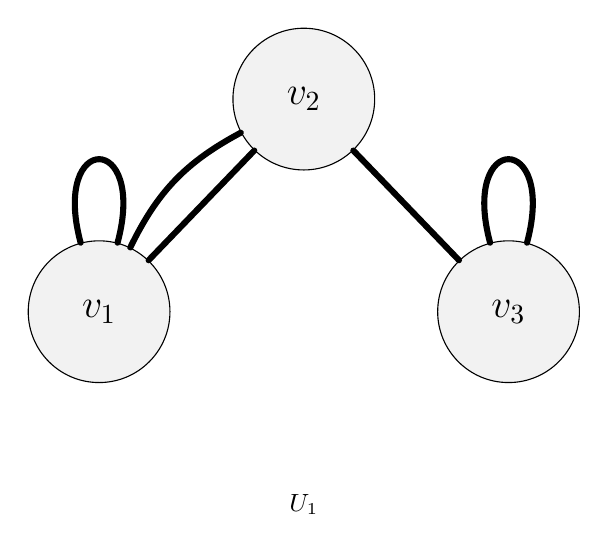
\begin{tikzpicture}[
  ugv/.style={circle, draw=black, fill=gray!10, minimum size=18.0mm, inner sep=2.0pt, font={\Large}},
  ugedge/.style={line width=2.20pt, line cap=round}
]
\node[ugv] (u0) at (-2.60,0.00) {$v_{1}$};
\node[ugv] (u1) at (0.00,2.70) {$v_{2}$};
\node[ugv] (u2) at (2.60,0.00) {$v_{3}$};
\draw[ugedge] (u0) to[loop above] (u0);
\draw[ugedge] (u0) -- (u1);
\draw[ugedge] (u0) to[bend left=18] (u1);
\draw[ugedge] (u1) -- (u2);
\draw[ugedge] (u2) to[loop above] (u2);
\node[font={\small}] at (0,-2.45) {$U_1$};
\end{tikzpicture}%
}
\end{center}
\item $U_2$.
\begin{center}
\resizebox{0.52\linewidth}{!}{%
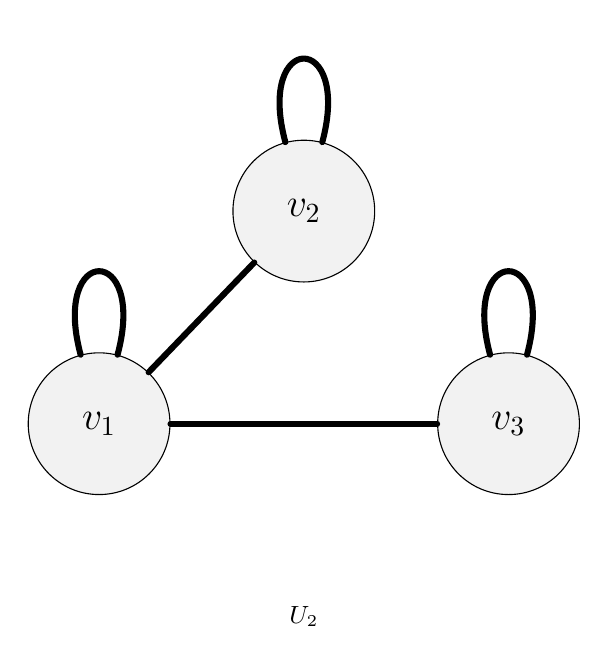
\begin{tikzpicture}[
  ugv/.style={circle, draw=black, fill=gray!10, minimum size=18.0mm, inner sep=2.0pt, font={\Large}},
  ugedge/.style={line width=2.20pt, line cap=round}
]
\node[ugv] (u0) at (-2.60,0.00) {$v_{1}$};
\node[ugv] (u1) at (0.00,2.70) {$v_{2}$};
\node[ugv] (u2) at (2.60,0.00) {$v_{3}$};
\draw[ugedge] (u0) to[loop above] (u0);
\draw[ugedge] (u0) -- (u1);
\draw[ugedge] (u0) -- (u2);
\draw[ugedge] (u1) to[loop above] (u1);
\draw[ugedge] (u2) to[loop above] (u2);
\node[font={\small}] at (0,-2.45) {$U_2$};
\end{tikzpicture}%
}
\end{center}
\item $U_3$.
\begin{center}
\resizebox{0.52\linewidth}{!}{%
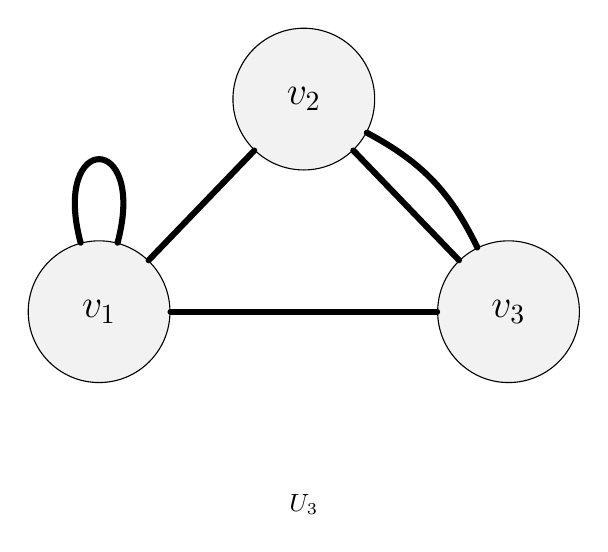
\begin{tikzpicture}[
  ugv/.style={circle, draw=black, fill=gray!10, minimum size=18.0mm, inner sep=2.0pt, font={\Large}},
  ugedge/.style={line width=2.20pt, line cap=round}
]
\node[ugv] (u0) at (-2.60,0.00) {$v_{1}$};
\node[ugv] (u1) at (0.00,2.70) {$v_{2}$};
\node[ugv] (u2) at (2.60,0.00) {$v_{3}$};
\draw[ugedge] (u0) to[loop above] (u0);
\draw[ugedge] (u0) -- (u1);
\draw[ugedge] (u0) -- (u2);
\draw[ugedge] (u1) -- (u2);
\draw[ugedge] (u1) to[bend left=18] (u2);
\node[font={\small}] at (0,-2.45) {$U_3$};
\end{tikzpicture}%
}
\end{center}
\item $U_4$.
\begin{center}
\resizebox{0.52\linewidth}{!}{%
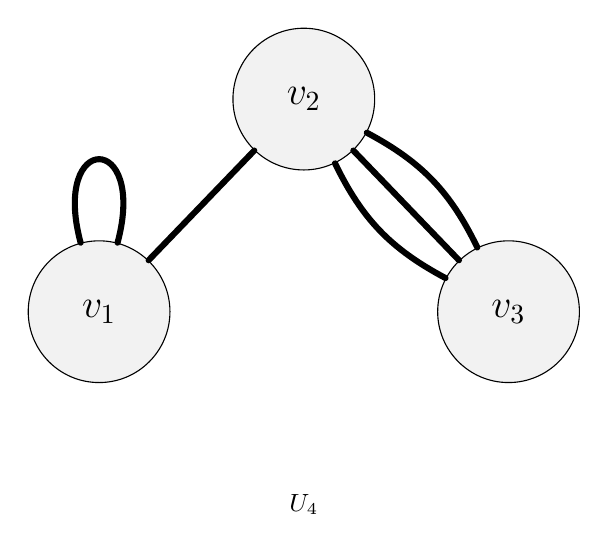
\begin{tikzpicture}[
  ugv/.style={circle, draw=black, fill=gray!10, minimum size=18.0mm, inner sep=2.0pt, font={\Large}},
  ugedge/.style={line width=2.20pt, line cap=round}
]
\node[ugv] (u0) at (-2.60,0.00) {$v_{1}$};
\node[ugv] (u1) at (0.00,2.70) {$v_{2}$};
\node[ugv] (u2) at (2.60,0.00) {$v_{3}$};
\draw[ugedge] (u0) to[loop above] (u0);
\draw[ugedge] (u0) -- (u1);
\draw[ugedge] (u1) -- (u2);
\draw[ugedge] (u1) to[bend left=18] (u2);
\draw[ugedge] (u1) to[bend right=18] (u2);
\node[font={\small}] at (0,-2.45) {$U_4$};
\end{tikzpicture}%
}
\end{center}
\item $U_5$.
\begin{center}
\resizebox{0.52\linewidth}{!}{%
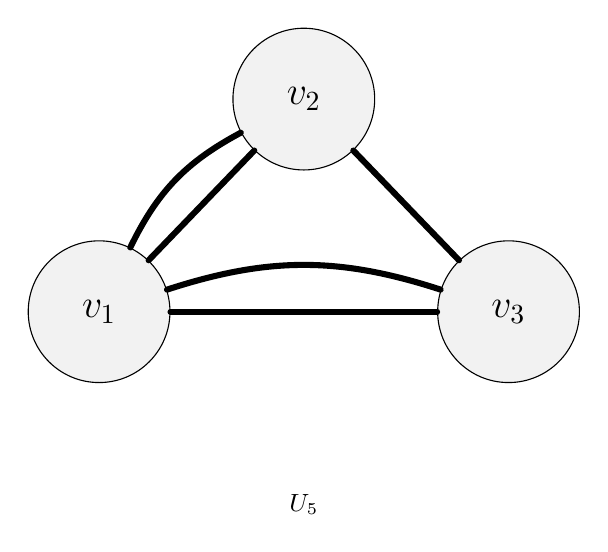
\begin{tikzpicture}[
  ugv/.style={circle, draw=black, fill=gray!10, minimum size=18.0mm, inner sep=2.0pt, font={\Large}},
  ugedge/.style={line width=2.20pt, line cap=round}
]
\node[ugv] (u0) at (-2.60,0.00) {$v_{1}$};
\node[ugv] (u1) at (0.00,2.70) {$v_{2}$};
\node[ugv] (u2) at (2.60,0.00) {$v_{3}$};
\draw[ugedge] (u0) -- (u1);
\draw[ugedge] (u0) to[bend left=18] (u1);
\draw[ugedge] (u0) -- (u2);
\draw[ugedge] (u0) to[bend left=18] (u2);
\draw[ugedge] (u1) -- (u2);
\node[font={\small}] at (0,-2.45) {$U_5$};
\end{tikzpicture}%
}
\end{center}
\end{enumerate}

\subsection*{Dictionary of graph labels used in preAUT/AUT}
For each graph label used above, this table records the corresponding ltt structure data.

\begin{enumerate}[leftmargin=*]
\item $G$:
\begin{itemize}[leftmargin=*]
\item underlying graph class $= U_5$.
\item red vertex $= x_{1}$.
\item red edge $= \{x_{1},\,\bar{x}_{5}\}$.
\item purple edges ($|\mathcal{P}|=9$):\mbox{}\\
$P_{1}: \{x_{2},\,x_{4}\},\; \{x_{2},\,x_{5}\},\; \{x_{4},\,x_{5}\}$\\
$P_{2}: \{x_{3},\,\bar{x}_{1}\},\; \{x_{3},\,\bar{x}_{2}\},\; \{\bar{x}_{1},\,\bar{x}_{2}\}$\\
$P_{3}: \{\bar{x}_{3},\,\bar{x}_{4}\},\; \{\bar{x}_{3},\,\bar{x}_{5}\},\; \{\bar{x}_{4},\,\bar{x}_{5}\}$.
\item black edges ($|\mathcal{B}|=5$): $\{x_{1},\,\bar{x}_{1}\},\; \{x_{2},\,\bar{x}_{2}\},\; \{x_{3},\,\bar{x}_{3}\},\; \{x_{4},\,\bar{x}_{4}\},\; \{x_{5},\,\bar{x}_{5}\}$.
\end{itemize}
\item $G_{1}$:
\begin{itemize}[leftmargin=*]
\item underlying graph class $= U_3$.
\item red vertex $= x_{1}$.
\item red edge $= \{x_{1},\,x_{3}\}$.
\item purple edges ($|\mathcal{P}|=9$):\mbox{}\\
$P_{1}: \{x_{2},\,x_{4}\},\; \{x_{2},\,x_{5}\},\; \{x_{4},\,x_{5}\}$\\
$P_{2}: \{x_{3},\,\bar{x}_{1}\},\; \{x_{3},\,\bar{x}_{2}\},\; \{\bar{x}_{1},\,\bar{x}_{2}\}$\\
$P_{3}: \{\bar{x}_{3},\,\bar{x}_{4}\},\; \{\bar{x}_{3},\,\bar{x}_{5}\},\; \{\bar{x}_{4},\,\bar{x}_{5}\}$.
\item black edges ($|\mathcal{B}|=5$): $\{x_{1},\,\bar{x}_{1}\},\; \{x_{2},\,\bar{x}_{2}\},\; \{x_{3},\,\bar{x}_{3}\},\; \{x_{4},\,\bar{x}_{4}\},\; \{x_{5},\,\bar{x}_{5}\}$.
\end{itemize}
\item $G_{2}$:
\begin{itemize}[leftmargin=*]
\item underlying graph class $= U_5$.
\item red vertex $= x_{1}$.
\item red edge $= \{x_{1},\,x_{4}\}$.
\item purple edges ($|\mathcal{P}|=9$):\mbox{}\\
$P_{1}: \{x_{2},\,x_{4}\},\; \{x_{2},\,x_{5}\},\; \{x_{4},\,x_{5}\}$\\
$P_{2}: \{x_{3},\,\bar{x}_{1}\},\; \{x_{3},\,\bar{x}_{2}\},\; \{\bar{x}_{1},\,\bar{x}_{2}\}$\\
$P_{3}: \{\bar{x}_{3},\,\bar{x}_{4}\},\; \{\bar{x}_{3},\,\bar{x}_{5}\},\; \{\bar{x}_{4},\,\bar{x}_{5}\}$.
\item black edges ($|\mathcal{B}|=5$): $\{x_{1},\,\bar{x}_{1}\},\; \{x_{2},\,\bar{x}_{2}\},\; \{x_{3},\,\bar{x}_{3}\},\; \{x_{4},\,\bar{x}_{4}\},\; \{x_{5},\,\bar{x}_{5}\}$.
\end{itemize}
\item $G_{3}$:
\begin{itemize}[leftmargin=*]
\item underlying graph class $= U_3$.
\item red vertex $= \bar{x}_{3}$.
\item red edge $= \{\bar{x}_{1},\,\bar{x}_{3}\}$.
\item purple edges ($|\mathcal{P}|=9$):\mbox{}\\
$P_{1}: \{x_{1},\,\bar{x}_{4}\},\; \{x_{1},\,\bar{x}_{5}\},\; \{\bar{x}_{4},\,\bar{x}_{5}\}$\\
$P_{2}: \{x_{2},\,x_{4}\},\; \{x_{2},\,x_{5}\},\; \{x_{4},\,x_{5}\}$\\
$P_{3}: \{x_{3},\,\bar{x}_{1}\},\; \{x_{3},\,\bar{x}_{2}\},\; \{\bar{x}_{1},\,\bar{x}_{2}\}$.
\item black edges ($|\mathcal{B}|=5$): $\{x_{1},\,\bar{x}_{1}\},\; \{x_{2},\,\bar{x}_{2}\},\; \{x_{3},\,\bar{x}_{3}\},\; \{x_{4},\,\bar{x}_{4}\},\; \{x_{5},\,\bar{x}_{5}\}$.
\end{itemize}
\item $G_{4}$:
\begin{itemize}[leftmargin=*]
\item underlying graph class $= U_5$.
\item red vertex $= \bar{x}_{4}$.
\item red edge $= \{\bar{x}_{1},\,\bar{x}_{4}\}$.
\item purple edges ($|\mathcal{P}|=9$):\mbox{}\\
$P_{1}: \{x_{1},\,\bar{x}_{3}\},\; \{x_{1},\,\bar{x}_{5}\},\; \{\bar{x}_{3},\,\bar{x}_{5}\}$\\
$P_{2}: \{x_{2},\,x_{4}\},\; \{x_{2},\,x_{5}\},\; \{x_{4},\,x_{5}\}$\\
$P_{3}: \{x_{3},\,\bar{x}_{1}\},\; \{x_{3},\,\bar{x}_{2}\},\; \{\bar{x}_{1},\,\bar{x}_{2}\}$.
\item black edges ($|\mathcal{B}|=5$): $\{x_{1},\,\bar{x}_{1}\},\; \{x_{2},\,\bar{x}_{2}\},\; \{x_{3},\,\bar{x}_{3}\},\; \{x_{4},\,\bar{x}_{4}\},\; \{x_{5},\,\bar{x}_{5}\}$.
\end{itemize}
\item $G_{5}$:
\begin{itemize}[leftmargin=*]
\item underlying graph class $= U_5$.
\item red vertex $= x_{1}$.
\item red edge $= \{x_{1},\,x_{2}\}$.
\item purple edges ($|\mathcal{P}|=9$):\mbox{}\\
$P_{1}: \{x_{2},\,x_{4}\},\; \{x_{2},\,x_{5}\},\; \{x_{4},\,x_{5}\}$\\
$P_{2}: \{x_{3},\,\bar{x}_{1}\},\; \{x_{3},\,\bar{x}_{2}\},\; \{\bar{x}_{1},\,\bar{x}_{2}\}$\\
$P_{3}: \{\bar{x}_{3},\,\bar{x}_{4}\},\; \{\bar{x}_{3},\,\bar{x}_{5}\},\; \{\bar{x}_{4},\,\bar{x}_{5}\}$.
\item black edges ($|\mathcal{B}|=5$): $\{x_{1},\,\bar{x}_{1}\},\; \{x_{2},\,\bar{x}_{2}\},\; \{x_{3},\,\bar{x}_{3}\},\; \{x_{4},\,\bar{x}_{4}\},\; \{x_{5},\,\bar{x}_{5}\}$.
\end{itemize}
\item $G_{6}$:
\begin{itemize}[leftmargin=*]
\item underlying graph class $= U_3$.
\item red vertex $= \bar{x}_{2}$.
\item red edge $= \{\bar{x}_{1},\,\bar{x}_{2}\}$.
\item purple edges ($|\mathcal{P}|=9$):\mbox{}\\
$P_{1}: \{x_{1},\,x_{3}\},\; \{x_{1},\,\bar{x}_{1}\},\; \{x_{3},\,\bar{x}_{1}\}$\\
$P_{2}: \{x_{2},\,x_{4}\},\; \{x_{2},\,x_{5}\},\; \{x_{4},\,x_{5}\}$\\
$P_{3}: \{\bar{x}_{3},\,\bar{x}_{4}\},\; \{\bar{x}_{3},\,\bar{x}_{5}\},\; \{\bar{x}_{4},\,\bar{x}_{5}\}$.
\item black edges ($|\mathcal{B}|=5$): $\{x_{1},\,\bar{x}_{1}\},\; \{x_{2},\,\bar{x}_{2}\},\; \{x_{3},\,\bar{x}_{3}\},\; \{x_{4},\,\bar{x}_{4}\},\; \{x_{5},\,\bar{x}_{5}\}$.
\end{itemize}
\item $G_{7}$:
\begin{itemize}[leftmargin=*]
\item underlying graph class $= U_5$.
\item red vertex $= x_{1}$.
\item red edge $= \{x_{1},\,\bar{x}_{4}\}$.
\item purple edges ($|\mathcal{P}|=9$):\mbox{}\\
$P_{1}: \{x_{2},\,x_{4}\},\; \{x_{2},\,x_{5}\},\; \{x_{4},\,x_{5}\}$\\
$P_{2}: \{x_{3},\,\bar{x}_{1}\},\; \{x_{3},\,\bar{x}_{2}\},\; \{\bar{x}_{1},\,\bar{x}_{2}\}$\\
$P_{3}: \{\bar{x}_{3},\,\bar{x}_{4}\},\; \{\bar{x}_{3},\,\bar{x}_{5}\},\; \{\bar{x}_{4},\,\bar{x}_{5}\}$.
\item black edges ($|\mathcal{B}|=5$): $\{x_{1},\,\bar{x}_{1}\},\; \{x_{2},\,\bar{x}_{2}\},\; \{x_{3},\,\bar{x}_{3}\},\; \{x_{4},\,\bar{x}_{4}\},\; \{x_{5},\,\bar{x}_{5}\}$.
\end{itemize}
\item $G_{8}$:
\begin{itemize}[leftmargin=*]
\item underlying graph class $= U_5$.
\item red vertex $= x_{4}$.
\item red edge $= \{x_{4},\,\bar{x}_{1}\}$.
\item purple edges ($|\mathcal{P}|=9$):\mbox{}\\
$P_{1}: \{x_{1},\,x_{2}\},\; \{x_{1},\,x_{5}\},\; \{x_{2},\,x_{5}\}$\\
$P_{2}: \{x_{3},\,\bar{x}_{1}\},\; \{x_{3},\,\bar{x}_{2}\},\; \{\bar{x}_{1},\,\bar{x}_{2}\}$\\
$P_{3}: \{\bar{x}_{3},\,\bar{x}_{4}\},\; \{\bar{x}_{3},\,\bar{x}_{5}\},\; \{\bar{x}_{4},\,\bar{x}_{5}\}$.
\item black edges ($|\mathcal{B}|=5$): $\{x_{1},\,\bar{x}_{1}\},\; \{x_{2},\,\bar{x}_{2}\},\; \{x_{3},\,\bar{x}_{3}\},\; \{x_{4},\,\bar{x}_{4}\},\; \{x_{5},\,\bar{x}_{5}\}$.
\end{itemize}
\item $G_{9}$:
\begin{itemize}[leftmargin=*]
\item underlying graph class $= U_5$.
\item red vertex $= x_{5}$.
\item red edge $= \{x_{5},\,\bar{x}_{1}\}$.
\item purple edges ($|\mathcal{P}|=9$):\mbox{}\\
$P_{1}: \{x_{1},\,x_{2}\},\; \{x_{1},\,x_{4}\},\; \{x_{2},\,x_{4}\}$\\
$P_{2}: \{x_{3},\,\bar{x}_{1}\},\; \{x_{3},\,\bar{x}_{2}\},\; \{\bar{x}_{1},\,\bar{x}_{2}\}$\\
$P_{3}: \{\bar{x}_{3},\,\bar{x}_{4}\},\; \{\bar{x}_{3},\,\bar{x}_{5}\},\; \{\bar{x}_{4},\,\bar{x}_{5}\}$.
\item black edges ($|\mathcal{B}|=5$): $\{x_{1},\,\bar{x}_{1}\},\; \{x_{2},\,\bar{x}_{2}\},\; \{x_{3},\,\bar{x}_{3}\},\; \{x_{4},\,\bar{x}_{4}\},\; \{x_{5},\,\bar{x}_{5}\}$.
\end{itemize}
\item $G_{10}$:
\begin{itemize}[leftmargin=*]
\item underlying graph class $= U_4$.
\item red vertex $= x_{3}$.
\item red edge $= \{x_{2},\,x_{3}\}$.
\item purple edges ($|\mathcal{P}|=9$):\mbox{}\\
$P_{1}: \{x_{1},\,\bar{x}_{1}\},\; \{x_{1},\,\bar{x}_{2}\},\; \{\bar{x}_{1},\,\bar{x}_{2}\}$\\
$P_{2}: \{x_{2},\,x_{4}\},\; \{x_{2},\,x_{5}\},\; \{x_{4},\,x_{5}\}$\\
$P_{3}: \{\bar{x}_{3},\,\bar{x}_{4}\},\; \{\bar{x}_{3},\,\bar{x}_{5}\},\; \{\bar{x}_{4},\,\bar{x}_{5}\}$.
\item black edges ($|\mathcal{B}|=5$): $\{x_{1},\,\bar{x}_{1}\},\; \{x_{2},\,\bar{x}_{2}\},\; \{x_{3},\,\bar{x}_{3}\},\; \{x_{4},\,\bar{x}_{4}\},\; \{x_{5},\,\bar{x}_{5}\}$.
\end{itemize}
\item $G_{11}$:
\begin{itemize}[leftmargin=*]
\item underlying graph class $= U_4$.
\item red vertex $= \bar{x}_{2}$.
\item red edge $= \{\bar{x}_{2},\,\bar{x}_{3}\}$.
\item purple edges ($|\mathcal{P}|=9$):\mbox{}\\
$P_{1}: \{x_{1},\,x_{3}\},\; \{x_{1},\,\bar{x}_{1}\},\; \{x_{3},\,\bar{x}_{1}\}$\\
$P_{2}: \{x_{2},\,x_{4}\},\; \{x_{2},\,x_{5}\},\; \{x_{4},\,x_{5}\}$\\
$P_{3}: \{\bar{x}_{3},\,\bar{x}_{4}\},\; \{\bar{x}_{3},\,\bar{x}_{5}\},\; \{\bar{x}_{4},\,\bar{x}_{5}\}$.
\item black edges ($|\mathcal{B}|=5$): $\{x_{1},\,\bar{x}_{1}\},\; \{x_{2},\,\bar{x}_{2}\},\; \{x_{3},\,\bar{x}_{3}\},\; \{x_{4},\,\bar{x}_{4}\},\; \{x_{5},\,\bar{x}_{5}\}$.
\end{itemize}
\item $G_{12}$:
\begin{itemize}[leftmargin=*]
\item underlying graph class $= U_1$.
\item red vertex $= x_{3}$.
\item red edge $= \{x_{3},\,\bar{x}_{4}\}$.
\item purple edges ($|\mathcal{P}|=9$):\mbox{}\\
$P_{1}: \{x_{1},\,\bar{x}_{1}\},\; \{x_{1},\,\bar{x}_{2}\},\; \{\bar{x}_{1},\,\bar{x}_{2}\}$\\
$P_{2}: \{x_{2},\,x_{4}\},\; \{x_{2},\,x_{5}\},\; \{x_{4},\,x_{5}\}$\\
$P_{3}: \{\bar{x}_{3},\,\bar{x}_{4}\},\; \{\bar{x}_{3},\,\bar{x}_{5}\},\; \{\bar{x}_{4},\,\bar{x}_{5}\}$.
\item black edges ($|\mathcal{B}|=5$): $\{x_{1},\,\bar{x}_{1}\},\; \{x_{2},\,\bar{x}_{2}\},\; \{x_{3},\,\bar{x}_{3}\},\; \{x_{4},\,\bar{x}_{4}\},\; \{x_{5},\,\bar{x}_{5}\}$.
\end{itemize}
\item $G_{13}$:
\begin{itemize}[leftmargin=*]
\item underlying graph class $= U_1$.
\item red vertex $= x_{3}$.
\item red edge $= \{x_{3},\,\bar{x}_{5}\}$.
\item purple edges ($|\mathcal{P}|=9$):\mbox{}\\
$P_{1}: \{x_{1},\,\bar{x}_{1}\},\; \{x_{1},\,\bar{x}_{2}\},\; \{\bar{x}_{1},\,\bar{x}_{2}\}$\\
$P_{2}: \{x_{2},\,x_{4}\},\; \{x_{2},\,x_{5}\},\; \{x_{4},\,x_{5}\}$\\
$P_{3}: \{\bar{x}_{3},\,\bar{x}_{4}\},\; \{\bar{x}_{3},\,\bar{x}_{5}\},\; \{\bar{x}_{4},\,\bar{x}_{5}\}$.
\item black edges ($|\mathcal{B}|=5$): $\{x_{1},\,\bar{x}_{1}\},\; \{x_{2},\,\bar{x}_{2}\},\; \{x_{3},\,\bar{x}_{3}\},\; \{x_{4},\,\bar{x}_{4}\},\; \{x_{5},\,\bar{x}_{5}\}$.
\end{itemize}
\item $G_{14}$:
\begin{itemize}[leftmargin=*]
\item underlying graph class $= U_1$.
\item red vertex $= x_{4}$.
\item red edge $= \{x_{4},\,\bar{x}_{3}\}$.
\item purple edges ($|\mathcal{P}|=9$):\mbox{}\\
$P_{1}: \{x_{1},\,\bar{x}_{1}\},\; \{x_{1},\,\bar{x}_{2}\},\; \{\bar{x}_{1},\,\bar{x}_{2}\}$\\
$P_{2}: \{x_{2},\,x_{3}\},\; \{x_{2},\,x_{5}\},\; \{x_{3},\,x_{5}\}$\\
$P_{3}: \{\bar{x}_{3},\,\bar{x}_{4}\},\; \{\bar{x}_{3},\,\bar{x}_{5}\},\; \{\bar{x}_{4},\,\bar{x}_{5}\}$.
\item black edges ($|\mathcal{B}|=5$): $\{x_{1},\,\bar{x}_{1}\},\; \{x_{2},\,\bar{x}_{2}\},\; \{x_{3},\,\bar{x}_{3}\},\; \{x_{4},\,\bar{x}_{4}\},\; \{x_{5},\,\bar{x}_{5}\}$.
\end{itemize}
\item $G_{15}$:
\begin{itemize}[leftmargin=*]
\item underlying graph class $= U_1$.
\item red vertex $= x_{5}$.
\item red edge $= \{x_{5},\,\bar{x}_{3}\}$.
\item purple edges ($|\mathcal{P}|=9$):\mbox{}\\
$P_{1}: \{x_{1},\,\bar{x}_{1}\},\; \{x_{1},\,\bar{x}_{2}\},\; \{\bar{x}_{1},\,\bar{x}_{2}\}$\\
$P_{2}: \{x_{2},\,x_{3}\},\; \{x_{2},\,x_{4}\},\; \{x_{3},\,x_{4}\}$\\
$P_{3}: \{\bar{x}_{3},\,\bar{x}_{4}\},\; \{\bar{x}_{3},\,\bar{x}_{5}\},\; \{\bar{x}_{4},\,\bar{x}_{5}\}$.
\item black edges ($|\mathcal{B}|=5$): $\{x_{1},\,\bar{x}_{1}\},\; \{x_{2},\,\bar{x}_{2}\},\; \{x_{3},\,\bar{x}_{3}\},\; \{x_{4},\,\bar{x}_{4}\},\; \{x_{5},\,\bar{x}_{5}\}$.
\end{itemize}
\item $G_{16}$:
\begin{itemize}[leftmargin=*]
\item underlying graph class $= U_4$.
\item red vertex $= x_{3}$.
\item red edge $= \{x_{3},\,x_{5}\}$.
\item purple edges ($|\mathcal{P}|=9$):\mbox{}\\
$P_{1}: \{x_{1},\,\bar{x}_{1}\},\; \{x_{1},\,\bar{x}_{2}\},\; \{\bar{x}_{1},\,\bar{x}_{2}\}$\\
$P_{2}: \{x_{2},\,x_{4}\},\; \{x_{2},\,x_{5}\},\; \{x_{4},\,x_{5}\}$\\
$P_{3}: \{\bar{x}_{3},\,\bar{x}_{4}\},\; \{\bar{x}_{3},\,\bar{x}_{5}\},\; \{\bar{x}_{4},\,\bar{x}_{5}\}$.
\item black edges ($|\mathcal{B}|=5$): $\{x_{1},\,\bar{x}_{1}\},\; \{x_{2},\,\bar{x}_{2}\},\; \{x_{3},\,\bar{x}_{3}\},\; \{x_{4},\,\bar{x}_{4}\},\; \{x_{5},\,\bar{x}_{5}\}$.
\end{itemize}
\item $G_{17}$:
\begin{itemize}[leftmargin=*]
\item underlying graph class $= U_1$.
\item red vertex $= \bar{x}_{5}$.
\item red edge $= \{\bar{x}_{3},\,\bar{x}_{5}\}$.
\item purple edges ($|\mathcal{P}|=9$):\mbox{}\\
$P_{1}: \{x_{1},\,\bar{x}_{1}\},\; \{x_{1},\,\bar{x}_{2}\},\; \{\bar{x}_{1},\,\bar{x}_{2}\}$\\
$P_{2}: \{x_{2},\,x_{4}\},\; \{x_{2},\,x_{5}\},\; \{x_{4},\,x_{5}\}$\\
$P_{3}: \{x_{3},\,\bar{x}_{3}\},\; \{x_{3},\,\bar{x}_{4}\},\; \{\bar{x}_{3},\,\bar{x}_{4}\}$.
\item black edges ($|\mathcal{B}|=5$): $\{x_{1},\,\bar{x}_{1}\},\; \{x_{2},\,\bar{x}_{2}\},\; \{x_{3},\,\bar{x}_{3}\},\; \{x_{4},\,\bar{x}_{4}\},\; \{x_{5},\,\bar{x}_{5}\}$.
\end{itemize}
\item $G_{18}$:
\begin{itemize}[leftmargin=*]
\item underlying graph class $= U_4$.
\item red vertex $= x_{2}$.
\item red edge $= \{x_{2},\,\bar{x}_{3}\}$.
\item purple edges ($|\mathcal{P}|=9$):\mbox{}\\
$P_{1}: \{x_{1},\,\bar{x}_{1}\},\; \{x_{1},\,\bar{x}_{2}\},\; \{\bar{x}_{1},\,\bar{x}_{2}\}$\\
$P_{2}: \{x_{3},\,x_{4}\},\; \{x_{3},\,x_{5}\},\; \{x_{4},\,x_{5}\}$\\
$P_{3}: \{\bar{x}_{3},\,\bar{x}_{4}\},\; \{\bar{x}_{3},\,\bar{x}_{5}\},\; \{\bar{x}_{4},\,\bar{x}_{5}\}$.
\item black edges ($|\mathcal{B}|=5$): $\{x_{1},\,\bar{x}_{1}\},\; \{x_{2},\,\bar{x}_{2}\},\; \{x_{3},\,\bar{x}_{3}\},\; \{x_{4},\,\bar{x}_{4}\},\; \{x_{5},\,\bar{x}_{5}\}$.
\end{itemize}
\item $G_{19}$:
\begin{itemize}[leftmargin=*]
\item underlying graph class $= U_3$.
\item red vertex $= x_{3}$.
\item red edge $= \{x_{3},\,\bar{x}_{2}\}$.
\item purple edges ($|\mathcal{P}|=9$):\mbox{}\\
$P_{1}: \{x_{1},\,\bar{x}_{1}\},\; \{x_{1},\,\bar{x}_{2}\},\; \{\bar{x}_{1},\,\bar{x}_{2}\}$\\
$P_{2}: \{x_{2},\,x_{4}\},\; \{x_{2},\,x_{5}\},\; \{x_{4},\,x_{5}\}$\\
$P_{3}: \{\bar{x}_{3},\,\bar{x}_{4}\},\; \{\bar{x}_{3},\,\bar{x}_{5}\},\; \{\bar{x}_{4},\,\bar{x}_{5}\}$.
\item black edges ($|\mathcal{B}|=5$): $\{x_{1},\,\bar{x}_{1}\},\; \{x_{2},\,\bar{x}_{2}\},\; \{x_{3},\,\bar{x}_{3}\},\; \{x_{4},\,\bar{x}_{4}\},\; \{x_{5},\,\bar{x}_{5}\}$.
\end{itemize}
\item $G_{20}$:
\begin{itemize}[leftmargin=*]
\item underlying graph class $= U_2$.
\item red vertex $= \bar{x}_{4}$.
\item red edge $= \{x_{5},\,\bar{x}_{4}\}$.
\item purple edges ($|\mathcal{P}|=9$):\mbox{}\\
$P_{1}: \{x_{1},\,\bar{x}_{1}\},\; \{x_{1},\,\bar{x}_{2}\},\; \{\bar{x}_{1},\,\bar{x}_{2}\}$\\
$P_{2}: \{x_{2},\,x_{4}\},\; \{x_{2},\,x_{5}\},\; \{x_{4},\,x_{5}\}$\\
$P_{3}: \{x_{3},\,\bar{x}_{3}\},\; \{x_{3},\,\bar{x}_{5}\},\; \{\bar{x}_{3},\,\bar{x}_{5}\}$.
\item black edges ($|\mathcal{B}|=5$): $\{x_{1},\,\bar{x}_{1}\},\; \{x_{2},\,\bar{x}_{2}\},\; \{x_{3},\,\bar{x}_{3}\},\; \{x_{4},\,\bar{x}_{4}\},\; \{x_{5},\,\bar{x}_{5}\}$.
\end{itemize}
\item $G_{21}$:
\begin{itemize}[leftmargin=*]
\item underlying graph class $= U_2$.
\item red vertex $= \bar{x}_{5}$.
\item red edge $= \{x_{4},\,\bar{x}_{5}\}$.
\item purple edges ($|\mathcal{P}|=9$):\mbox{}\\
$P_{1}: \{x_{1},\,\bar{x}_{1}\},\; \{x_{1},\,\bar{x}_{2}\},\; \{\bar{x}_{1},\,\bar{x}_{2}\}$\\
$P_{2}: \{x_{2},\,x_{4}\},\; \{x_{2},\,x_{5}\},\; \{x_{4},\,x_{5}\}$\\
$P_{3}: \{x_{3},\,\bar{x}_{3}\},\; \{x_{3},\,\bar{x}_{4}\},\; \{\bar{x}_{3},\,\bar{x}_{4}\}$.
\item black edges ($|\mathcal{B}|=5$): $\{x_{1},\,\bar{x}_{1}\},\; \{x_{2},\,\bar{x}_{2}\},\; \{x_{3},\,\bar{x}_{3}\},\; \{x_{4},\,\bar{x}_{4}\},\; \{x_{5},\,\bar{x}_{5}\}$.
\end{itemize}
\item $G_{22}$:
\begin{itemize}[leftmargin=*]
\item underlying graph class $= U_4$.
\item red vertex $= x_{2}$.
\item red edge $= \{x_{2},\,x_{4}\}$.
\item purple edges ($|\mathcal{P}|=9$):\mbox{}\\
$P_{1}: \{x_{1},\,\bar{x}_{1}\},\; \{x_{1},\,\bar{x}_{2}\},\; \{\bar{x}_{1},\,\bar{x}_{2}\}$\\
$P_{2}: \{x_{3},\,x_{4}\},\; \{x_{3},\,x_{5}\},\; \{x_{4},\,x_{5}\}$\\
$P_{3}: \{\bar{x}_{3},\,\bar{x}_{4}\},\; \{\bar{x}_{3},\,\bar{x}_{5}\},\; \{\bar{x}_{4},\,\bar{x}_{5}\}$.
\item black edges ($|\mathcal{B}|=5$): $\{x_{1},\,\bar{x}_{1}\},\; \{x_{2},\,\bar{x}_{2}\},\; \{x_{3},\,\bar{x}_{3}\},\; \{x_{4},\,\bar{x}_{4}\},\; \{x_{5},\,\bar{x}_{5}\}$.
\end{itemize}
\item $G_{23}$:
\begin{itemize}[leftmargin=*]
\item underlying graph class $= U_4$.
\item red vertex $= x_{2}$.
\item red edge $= \{x_{2},\,x_{5}\}$.
\item purple edges ($|\mathcal{P}|=9$):\mbox{}\\
$P_{1}: \{x_{1},\,\bar{x}_{1}\},\; \{x_{1},\,\bar{x}_{2}\},\; \{\bar{x}_{1},\,\bar{x}_{2}\}$\\
$P_{2}: \{x_{3},\,x_{4}\},\; \{x_{3},\,x_{5}\},\; \{x_{4},\,x_{5}\}$\\
$P_{3}: \{\bar{x}_{3},\,\bar{x}_{4}\},\; \{\bar{x}_{3},\,\bar{x}_{5}\},\; \{\bar{x}_{4},\,\bar{x}_{5}\}$.
\item black edges ($|\mathcal{B}|=5$): $\{x_{1},\,\bar{x}_{1}\},\; \{x_{2},\,\bar{x}_{2}\},\; \{x_{3},\,\bar{x}_{3}\},\; \{x_{4},\,\bar{x}_{4}\},\; \{x_{5},\,\bar{x}_{5}\}$.
\end{itemize}
\item $G_{24}$:
\begin{itemize}[leftmargin=*]
\item underlying graph class $= U_3$.
\item red vertex $= \bar{x}_{4}$.
\item red edge $= \{\bar{x}_{2},\,\bar{x}_{4}\}$.
\item purple edges ($|\mathcal{P}|=9$):\mbox{}\\
$P_{1}: \{x_{1},\,\bar{x}_{1}\},\; \{x_{1},\,\bar{x}_{2}\},\; \{\bar{x}_{1},\,\bar{x}_{2}\}$\\
$P_{2}: \{x_{2},\,\bar{x}_{3}\},\; \{x_{2},\,\bar{x}_{5}\},\; \{\bar{x}_{3},\,\bar{x}_{5}\}$\\
$P_{3}: \{x_{3},\,x_{4}\},\; \{x_{3},\,x_{5}\},\; \{x_{4},\,x_{5}\}$.
\item black edges ($|\mathcal{B}|=5$): $\{x_{1},\,\bar{x}_{1}\},\; \{x_{2},\,\bar{x}_{2}\},\; \{x_{3},\,\bar{x}_{3}\},\; \{x_{4},\,\bar{x}_{4}\},\; \{x_{5},\,\bar{x}_{5}\}$.
\end{itemize}
\item $G_{25}$:
\begin{itemize}[leftmargin=*]
\item underlying graph class $= U_3$.
\item red vertex $= \bar{x}_{5}$.
\item red edge $= \{\bar{x}_{2},\,\bar{x}_{5}\}$.
\item purple edges ($|\mathcal{P}|=9$):\mbox{}\\
$P_{1}: \{x_{1},\,\bar{x}_{1}\},\; \{x_{1},\,\bar{x}_{2}\},\; \{\bar{x}_{1},\,\bar{x}_{2}\}$\\
$P_{2}: \{x_{2},\,\bar{x}_{3}\},\; \{x_{2},\,\bar{x}_{4}\},\; \{\bar{x}_{3},\,\bar{x}_{4}\}$\\
$P_{3}: \{x_{3},\,x_{4}\},\; \{x_{3},\,x_{5}\},\; \{x_{4},\,x_{5}\}$.
\item black edges ($|\mathcal{B}|=5$): $\{x_{1},\,\bar{x}_{1}\},\; \{x_{2},\,\bar{x}_{2}\},\; \{x_{3},\,\bar{x}_{3}\},\; \{x_{4},\,\bar{x}_{4}\},\; \{x_{5},\,\bar{x}_{5}\}$.
\end{itemize}
\item $G_{26}$:
\begin{itemize}[leftmargin=*]
\item underlying graph class $= U_5$.
\item red vertex $= x_{1}$.
\item red edge $= \{x_{1},\,\bar{x}_{3}\}$.
\item purple edges ($|\mathcal{P}|=9$):\mbox{}\\
$P_{1}: \{x_{2},\,x_{4}\},\; \{x_{2},\,x_{5}\},\; \{x_{4},\,x_{5}\}$\\
$P_{2}: \{x_{3},\,\bar{x}_{1}\},\; \{x_{3},\,\bar{x}_{2}\},\; \{\bar{x}_{1},\,\bar{x}_{2}\}$\\
$P_{3}: \{\bar{x}_{3},\,\bar{x}_{4}\},\; \{\bar{x}_{3},\,\bar{x}_{5}\},\; \{\bar{x}_{4},\,\bar{x}_{5}\}$.
\item black edges ($|\mathcal{B}|=5$): $\{x_{1},\,\bar{x}_{1}\},\; \{x_{2},\,\bar{x}_{2}\},\; \{x_{3},\,\bar{x}_{3}\},\; \{x_{4},\,\bar{x}_{4}\},\; \{x_{5},\,\bar{x}_{5}\}$.
\end{itemize}
\item $G_{27}$:
\begin{itemize}[leftmargin=*]
\item underlying graph class $= U_3$.
\item red vertex $= x_{3}$.
\item red edge $= \{x_{1},\,x_{3}\}$.
\item purple edges ($|\mathcal{P}|=9$):\mbox{}\\
$P_{1}: \{x_{1},\,\bar{x}_{1}\},\; \{x_{1},\,\bar{x}_{2}\},\; \{\bar{x}_{1},\,\bar{x}_{2}\}$\\
$P_{2}: \{x_{2},\,x_{4}\},\; \{x_{2},\,x_{5}\},\; \{x_{4},\,x_{5}\}$\\
$P_{3}: \{\bar{x}_{3},\,\bar{x}_{4}\},\; \{\bar{x}_{3},\,\bar{x}_{5}\},\; \{\bar{x}_{4},\,\bar{x}_{5}\}$.
\item black edges ($|\mathcal{B}|=5$): $\{x_{1},\,\bar{x}_{1}\},\; \{x_{2},\,\bar{x}_{2}\},\; \{x_{3},\,\bar{x}_{3}\},\; \{x_{4},\,\bar{x}_{4}\},\; \{x_{5},\,\bar{x}_{5}\}$.
\end{itemize}
\item $G_{28}$:
\begin{itemize}[leftmargin=*]
\item underlying graph class $= U_3$.
\item red vertex $= x_{3}$.
\item red edge $= \{x_{3},\,\bar{x}_{1}\}$.
\item purple edges ($|\mathcal{P}|=9$):\mbox{}\\
$P_{1}: \{x_{1},\,\bar{x}_{1}\},\; \{x_{1},\,\bar{x}_{2}\},\; \{\bar{x}_{1},\,\bar{x}_{2}\}$\\
$P_{2}: \{x_{2},\,x_{4}\},\; \{x_{2},\,x_{5}\},\; \{x_{4},\,x_{5}\}$\\
$P_{3}: \{\bar{x}_{3},\,\bar{x}_{4}\},\; \{\bar{x}_{3},\,\bar{x}_{5}\},\; \{\bar{x}_{4},\,\bar{x}_{5}\}$.
\item black edges ($|\mathcal{B}|=5$): $\{x_{1},\,\bar{x}_{1}\},\; \{x_{2},\,\bar{x}_{2}\},\; \{x_{3},\,\bar{x}_{3}\},\; \{x_{4},\,\bar{x}_{4}\},\; \{x_{5},\,\bar{x}_{5}\}$.
\end{itemize}
\item $G_{29}$:
\begin{itemize}[leftmargin=*]
\item underlying graph class $= U_5$.
\item red vertex $= \bar{x}_{1}$.
\item red edge $= \{\bar{x}_{1},\,\bar{x}_{3}\}$.
\item purple edges ($|\mathcal{P}|=9$):\mbox{}\\
$P_{1}: \{x_{1},\,x_{3}\},\; \{x_{1},\,\bar{x}_{2}\},\; \{x_{3},\,\bar{x}_{2}\}$\\
$P_{2}: \{x_{2},\,x_{4}\},\; \{x_{2},\,x_{5}\},\; \{x_{4},\,x_{5}\}$\\
$P_{3}: \{\bar{x}_{3},\,\bar{x}_{4}\},\; \{\bar{x}_{3},\,\bar{x}_{5}\},\; \{\bar{x}_{4},\,\bar{x}_{5}\}$.
\item black edges ($|\mathcal{B}|=5$): $\{x_{1},\,\bar{x}_{1}\},\; \{x_{2},\,\bar{x}_{2}\},\; \{x_{3},\,\bar{x}_{3}\},\; \{x_{4},\,\bar{x}_{4}\},\; \{x_{5},\,\bar{x}_{5}\}$.
\end{itemize}
\item $G_{30}$:
\begin{itemize}[leftmargin=*]
\item underlying graph class $= U_2$.
\item red vertex $= x_{2}$.
\item red edge $= \{x_{2},\,x_{4}\}$.
\item purple edges ($|\mathcal{P}|=9$):\mbox{}\\
$P_{1}: \{x_{1},\,\bar{x}_{1}\},\; \{x_{1},\,\bar{x}_{2}\},\; \{\bar{x}_{1},\,\bar{x}_{2}\}$\\
$P_{2}: \{x_{3},\,\bar{x}_{3}\},\; \{x_{3},\,\bar{x}_{5}\},\; \{\bar{x}_{3},\,\bar{x}_{5}\}$\\
$P_{3}: \{x_{4},\,x_{5}\},\; \{x_{4},\,\bar{x}_{4}\},\; \{x_{5},\,\bar{x}_{4}\}$.
\item black edges ($|\mathcal{B}|=5$): $\{x_{1},\,\bar{x}_{1}\},\; \{x_{2},\,\bar{x}_{2}\},\; \{x_{3},\,\bar{x}_{3}\},\; \{x_{4},\,\bar{x}_{4}\},\; \{x_{5},\,\bar{x}_{5}\}$.
\end{itemize}
\item $G_{31}$:
\begin{itemize}[leftmargin=*]
\item underlying graph class $= U_1$.
\item red vertex $= \bar{x}_{4}$.
\item red edge $= \{\bar{x}_{2},\,\bar{x}_{4}\}$.
\item purple edges ($|\mathcal{P}|=9$):\mbox{}\\
$P_{1}: \{x_{1},\,\bar{x}_{1}\},\; \{x_{1},\,\bar{x}_{2}\},\; \{\bar{x}_{1},\,\bar{x}_{2}\}$\\
$P_{2}: \{x_{2},\,x_{4}\},\; \{x_{2},\,x_{5}\},\; \{x_{4},\,x_{5}\}$\\
$P_{3}: \{x_{3},\,\bar{x}_{3}\},\; \{x_{3},\,\bar{x}_{5}\},\; \{\bar{x}_{3},\,\bar{x}_{5}\}$.
\item black edges ($|\mathcal{B}|=5$): $\{x_{1},\,\bar{x}_{1}\},\; \{x_{2},\,\bar{x}_{2}\},\; \{x_{3},\,\bar{x}_{3}\},\; \{x_{4},\,\bar{x}_{4}\},\; \{x_{5},\,\bar{x}_{5}\}$.
\end{itemize}
\item $G_{32}$:
\begin{itemize}[leftmargin=*]
\item underlying graph class $= U_2$.
\item red vertex $= x_{2}$.
\item red edge $= \{x_{2},\,\bar{x}_{5}\}$.
\item purple edges ($|\mathcal{P}|=9$):\mbox{}\\
$P_{1}: \{x_{1},\,\bar{x}_{1}\},\; \{x_{1},\,\bar{x}_{2}\},\; \{\bar{x}_{1},\,\bar{x}_{2}\}$\\
$P_{2}: \{x_{3},\,\bar{x}_{3}\},\; \{x_{3},\,\bar{x}_{5}\},\; \{\bar{x}_{3},\,\bar{x}_{5}\}$\\
$P_{3}: \{x_{4},\,x_{5}\},\; \{x_{4},\,\bar{x}_{4}\},\; \{x_{5},\,\bar{x}_{4}\}$.
\item black edges ($|\mathcal{B}|=5$): $\{x_{1},\,\bar{x}_{1}\},\; \{x_{2},\,\bar{x}_{2}\},\; \{x_{3},\,\bar{x}_{3}\},\; \{x_{4},\,\bar{x}_{4}\},\; \{x_{5},\,\bar{x}_{5}\}$.
\end{itemize}
\item $G_{33}$:
\begin{itemize}[leftmargin=*]
\item underlying graph class $= U_2$.
\item red vertex $= x_{5}$.
\item red edge $= \{x_{5},\,\bar{x}_{2}\}$.
\item purple edges ($|\mathcal{P}|=9$):\mbox{}\\
$P_{1}: \{x_{1},\,\bar{x}_{1}\},\; \{x_{1},\,\bar{x}_{2}\},\; \{\bar{x}_{1},\,\bar{x}_{2}\}$\\
$P_{2}: \{x_{2},\,x_{4}\},\; \{x_{2},\,\bar{x}_{4}\},\; \{x_{4},\,\bar{x}_{4}\}$\\
$P_{3}: \{x_{3},\,\bar{x}_{3}\},\; \{x_{3},\,\bar{x}_{5}\},\; \{\bar{x}_{3},\,\bar{x}_{5}\}$.
\item black edges ($|\mathcal{B}|=5$): $\{x_{1},\,\bar{x}_{1}\},\; \{x_{2},\,\bar{x}_{2}\},\; \{x_{3},\,\bar{x}_{3}\},\; \{x_{4},\,\bar{x}_{4}\},\; \{x_{5},\,\bar{x}_{5}\}$.
\end{itemize}
\item $G_{34}$:
\begin{itemize}[leftmargin=*]
\item underlying graph class $= U_4$.
\item red vertex $= x_{1}$.
\item red edge $= \{x_{1},\,x_{4}\}$.
\item purple edges ($|\mathcal{P}|=9$):\mbox{}\\
$P_{1}: \{x_{2},\,x_{4}\},\; \{x_{2},\,x_{5}\},\; \{x_{4},\,x_{5}\}$\\
$P_{2}: \{x_{3},\,\bar{x}_{3}\},\; \{x_{3},\,\bar{x}_{5}\},\; \{\bar{x}_{3},\,\bar{x}_{5}\}$\\
$P_{3}: \{\bar{x}_{1},\,\bar{x}_{2}\},\; \{\bar{x}_{1},\,\bar{x}_{4}\},\; \{\bar{x}_{2},\,\bar{x}_{4}\}$.
\item black edges ($|\mathcal{B}|=5$): $\{x_{1},\,\bar{x}_{1}\},\; \{x_{2},\,\bar{x}_{2}\},\; \{x_{3},\,\bar{x}_{3}\},\; \{x_{4},\,\bar{x}_{4}\},\; \{x_{5},\,\bar{x}_{5}\}$.
\end{itemize}
\item $G_{35}$:
\begin{itemize}[leftmargin=*]
\item underlying graph class $= U_4$.
\item red vertex $= \bar{x}_{1}$.
\item red edge $= \{x_{4},\,\bar{x}_{1}\}$.
\item purple edges ($|\mathcal{P}|=9$):\mbox{}\\
$P_{1}: \{x_{1},\,\bar{x}_{2}\},\; \{x_{1},\,\bar{x}_{4}\},\; \{\bar{x}_{2},\,\bar{x}_{4}\}$\\
$P_{2}: \{x_{2},\,x_{4}\},\; \{x_{2},\,x_{5}\},\; \{x_{4},\,x_{5}\}$\\
$P_{3}: \{x_{3},\,\bar{x}_{3}\},\; \{x_{3},\,\bar{x}_{5}\},\; \{\bar{x}_{3},\,\bar{x}_{5}\}$.
\item black edges ($|\mathcal{B}|=5$): $\{x_{1},\,\bar{x}_{1}\},\; \{x_{2},\,\bar{x}_{2}\},\; \{x_{3},\,\bar{x}_{3}\},\; \{x_{4},\,\bar{x}_{4}\},\; \{x_{5},\,\bar{x}_{5}\}$.
\end{itemize}
\item $G_{36}$:
\begin{itemize}[leftmargin=*]
\item underlying graph class $= U_1$.
\item red vertex $= \bar{x}_{4}$.
\item red edge $= \{x_{1},\,\bar{x}_{4}\}$.
\item purple edges ($|\mathcal{P}|=9$):\mbox{}\\
$P_{1}: \{x_{1},\,\bar{x}_{1}\},\; \{x_{1},\,\bar{x}_{2}\},\; \{\bar{x}_{1},\,\bar{x}_{2}\}$\\
$P_{2}: \{x_{2},\,x_{4}\},\; \{x_{2},\,x_{5}\},\; \{x_{4},\,x_{5}\}$\\
$P_{3}: \{x_{3},\,\bar{x}_{3}\},\; \{x_{3},\,\bar{x}_{5}\},\; \{\bar{x}_{3},\,\bar{x}_{5}\}$.
\item black edges ($|\mathcal{B}|=5$): $\{x_{1},\,\bar{x}_{1}\},\; \{x_{2},\,\bar{x}_{2}\},\; \{x_{3},\,\bar{x}_{3}\},\; \{x_{4},\,\bar{x}_{4}\},\; \{x_{5},\,\bar{x}_{5}\}$.
\end{itemize}
\item $G_{37}$:
\begin{itemize}[leftmargin=*]
\item underlying graph class $= U_1$.
\item red vertex $= \bar{x}_{4}$.
\item red edge $= \{\bar{x}_{1},\,\bar{x}_{4}\}$.
\item purple edges ($|\mathcal{P}|=9$):\mbox{}\\
$P_{1}: \{x_{1},\,\bar{x}_{1}\},\; \{x_{1},\,\bar{x}_{2}\},\; \{\bar{x}_{1},\,\bar{x}_{2}\}$\\
$P_{2}: \{x_{2},\,x_{4}\},\; \{x_{2},\,x_{5}\},\; \{x_{4},\,x_{5}\}$\\
$P_{3}: \{x_{3},\,\bar{x}_{3}\},\; \{x_{3},\,\bar{x}_{5}\},\; \{\bar{x}_{3},\,\bar{x}_{5}\}$.
\item black edges ($|\mathcal{B}|=5$): $\{x_{1},\,\bar{x}_{1}\},\; \{x_{2},\,\bar{x}_{2}\},\; \{x_{3},\,\bar{x}_{3}\},\; \{x_{4},\,\bar{x}_{4}\},\; \{x_{5},\,\bar{x}_{5}\}$.
\end{itemize}
\item $G_{38}$:
\begin{itemize}[leftmargin=*]
\item underlying graph class $= U_2$.
\item red vertex $= x_{2}$.
\item red edge $= \{x_{2},\,x_{3}\}$.
\item purple edges ($|\mathcal{P}|=9$):\mbox{}\\
$P_{1}: \{x_{1},\,\bar{x}_{1}\},\; \{x_{1},\,\bar{x}_{2}\},\; \{\bar{x}_{1},\,\bar{x}_{2}\}$\\
$P_{2}: \{x_{3},\,\bar{x}_{3}\},\; \{x_{3},\,\bar{x}_{5}\},\; \{\bar{x}_{3},\,\bar{x}_{5}\}$\\
$P_{3}: \{x_{4},\,x_{5}\},\; \{x_{4},\,\bar{x}_{4}\},\; \{x_{5},\,\bar{x}_{4}\}$.
\item black edges ($|\mathcal{B}|=5$): $\{x_{1},\,\bar{x}_{1}\},\; \{x_{2},\,\bar{x}_{2}\},\; \{x_{3},\,\bar{x}_{3}\},\; \{x_{4},\,\bar{x}_{4}\},\; \{x_{5},\,\bar{x}_{5}\}$.
\end{itemize}
\item $G_{39}$:
\begin{itemize}[leftmargin=*]
\item underlying graph class $= U_2$.
\item red vertex $= x_{2}$.
\item red edge $= \{x_{2},\,\bar{x}_{3}\}$.
\item purple edges ($|\mathcal{P}|=9$):\mbox{}\\
$P_{1}: \{x_{1},\,\bar{x}_{1}\},\; \{x_{1},\,\bar{x}_{2}\},\; \{\bar{x}_{1},\,\bar{x}_{2}\}$\\
$P_{2}: \{x_{3},\,\bar{x}_{3}\},\; \{x_{3},\,\bar{x}_{5}\},\; \{\bar{x}_{3},\,\bar{x}_{5}\}$\\
$P_{3}: \{x_{4},\,x_{5}\},\; \{x_{4},\,\bar{x}_{4}\},\; \{x_{5},\,\bar{x}_{4}\}$.
\item black edges ($|\mathcal{B}|=5$): $\{x_{1},\,\bar{x}_{1}\},\; \{x_{2},\,\bar{x}_{2}\},\; \{x_{3},\,\bar{x}_{3}\},\; \{x_{4},\,\bar{x}_{4}\},\; \{x_{5},\,\bar{x}_{5}\}$.
\end{itemize}
\item $G_{40}$:
\begin{itemize}[leftmargin=*]
\item underlying graph class $= U_1$.
\item red vertex $= x_{3}$.
\item red edge $= \{x_{3},\,\bar{x}_{2}\}$.
\item purple edges ($|\mathcal{P}|=9$):\mbox{}\\
$P_{1}: \{x_{1},\,\bar{x}_{1}\},\; \{x_{1},\,\bar{x}_{2}\},\; \{\bar{x}_{1},\,\bar{x}_{2}\}$\\
$P_{2}: \{x_{2},\,\bar{x}_{3}\},\; \{x_{2},\,\bar{x}_{5}\},\; \{\bar{x}_{3},\,\bar{x}_{5}\}$\\
$P_{3}: \{x_{4},\,x_{5}\},\; \{x_{4},\,\bar{x}_{4}\},\; \{x_{5},\,\bar{x}_{4}\}$.
\item black edges ($|\mathcal{B}|=5$): $\{x_{1},\,\bar{x}_{1}\},\; \{x_{2},\,\bar{x}_{2}\},\; \{x_{3},\,\bar{x}_{3}\},\; \{x_{4},\,\bar{x}_{4}\},\; \{x_{5},\,\bar{x}_{5}\}$.
\end{itemize}
\item $G_{41}$:
\begin{itemize}[leftmargin=*]
\item underlying graph class $= U_1$.
\item red vertex $= \bar{x}_{3}$.
\item red edge $= \{\bar{x}_{2},\,\bar{x}_{3}\}$.
\item purple edges ($|\mathcal{P}|=9$):\mbox{}\\
$P_{1}: \{x_{1},\,\bar{x}_{1}\},\; \{x_{1},\,\bar{x}_{2}\},\; \{\bar{x}_{1},\,\bar{x}_{2}\}$\\
$P_{2}: \{x_{2},\,x_{3}\},\; \{x_{2},\,\bar{x}_{5}\},\; \{x_{3},\,\bar{x}_{5}\}$\\
$P_{3}: \{x_{4},\,x_{5}\},\; \{x_{4},\,\bar{x}_{4}\},\; \{x_{5},\,\bar{x}_{4}\}$.
\item black edges ($|\mathcal{B}|=5$): $\{x_{1},\,\bar{x}_{1}\},\; \{x_{2},\,\bar{x}_{2}\},\; \{x_{3},\,\bar{x}_{3}\},\; \{x_{4},\,\bar{x}_{4}\},\; \{x_{5},\,\bar{x}_{5}\}$.
\end{itemize}
\end{enumerate}

\subsection*{Visual depiction of AUT by component (box-collapsed)}
AUT is computed from the box-collapsed preAUT (one node per box). Retained AUT components are listed sequentially. Nodes are labeled by Roman box IDs (I--XIV). Blue (Step~2) edge labels count only non-permutation arrows along that directed box pair; green labels count permutation ($\varphi$) edges, so blue and green labels sum to the total parallel preAUT arrows between those boxes.

\clearpage
\paragraph{AUT component $\mathrm{SCC}_{1}$.}
\vfill
\begin{center}
\setbox0=\hbox{%
\resizebox{!}{0.96\textheight}{%
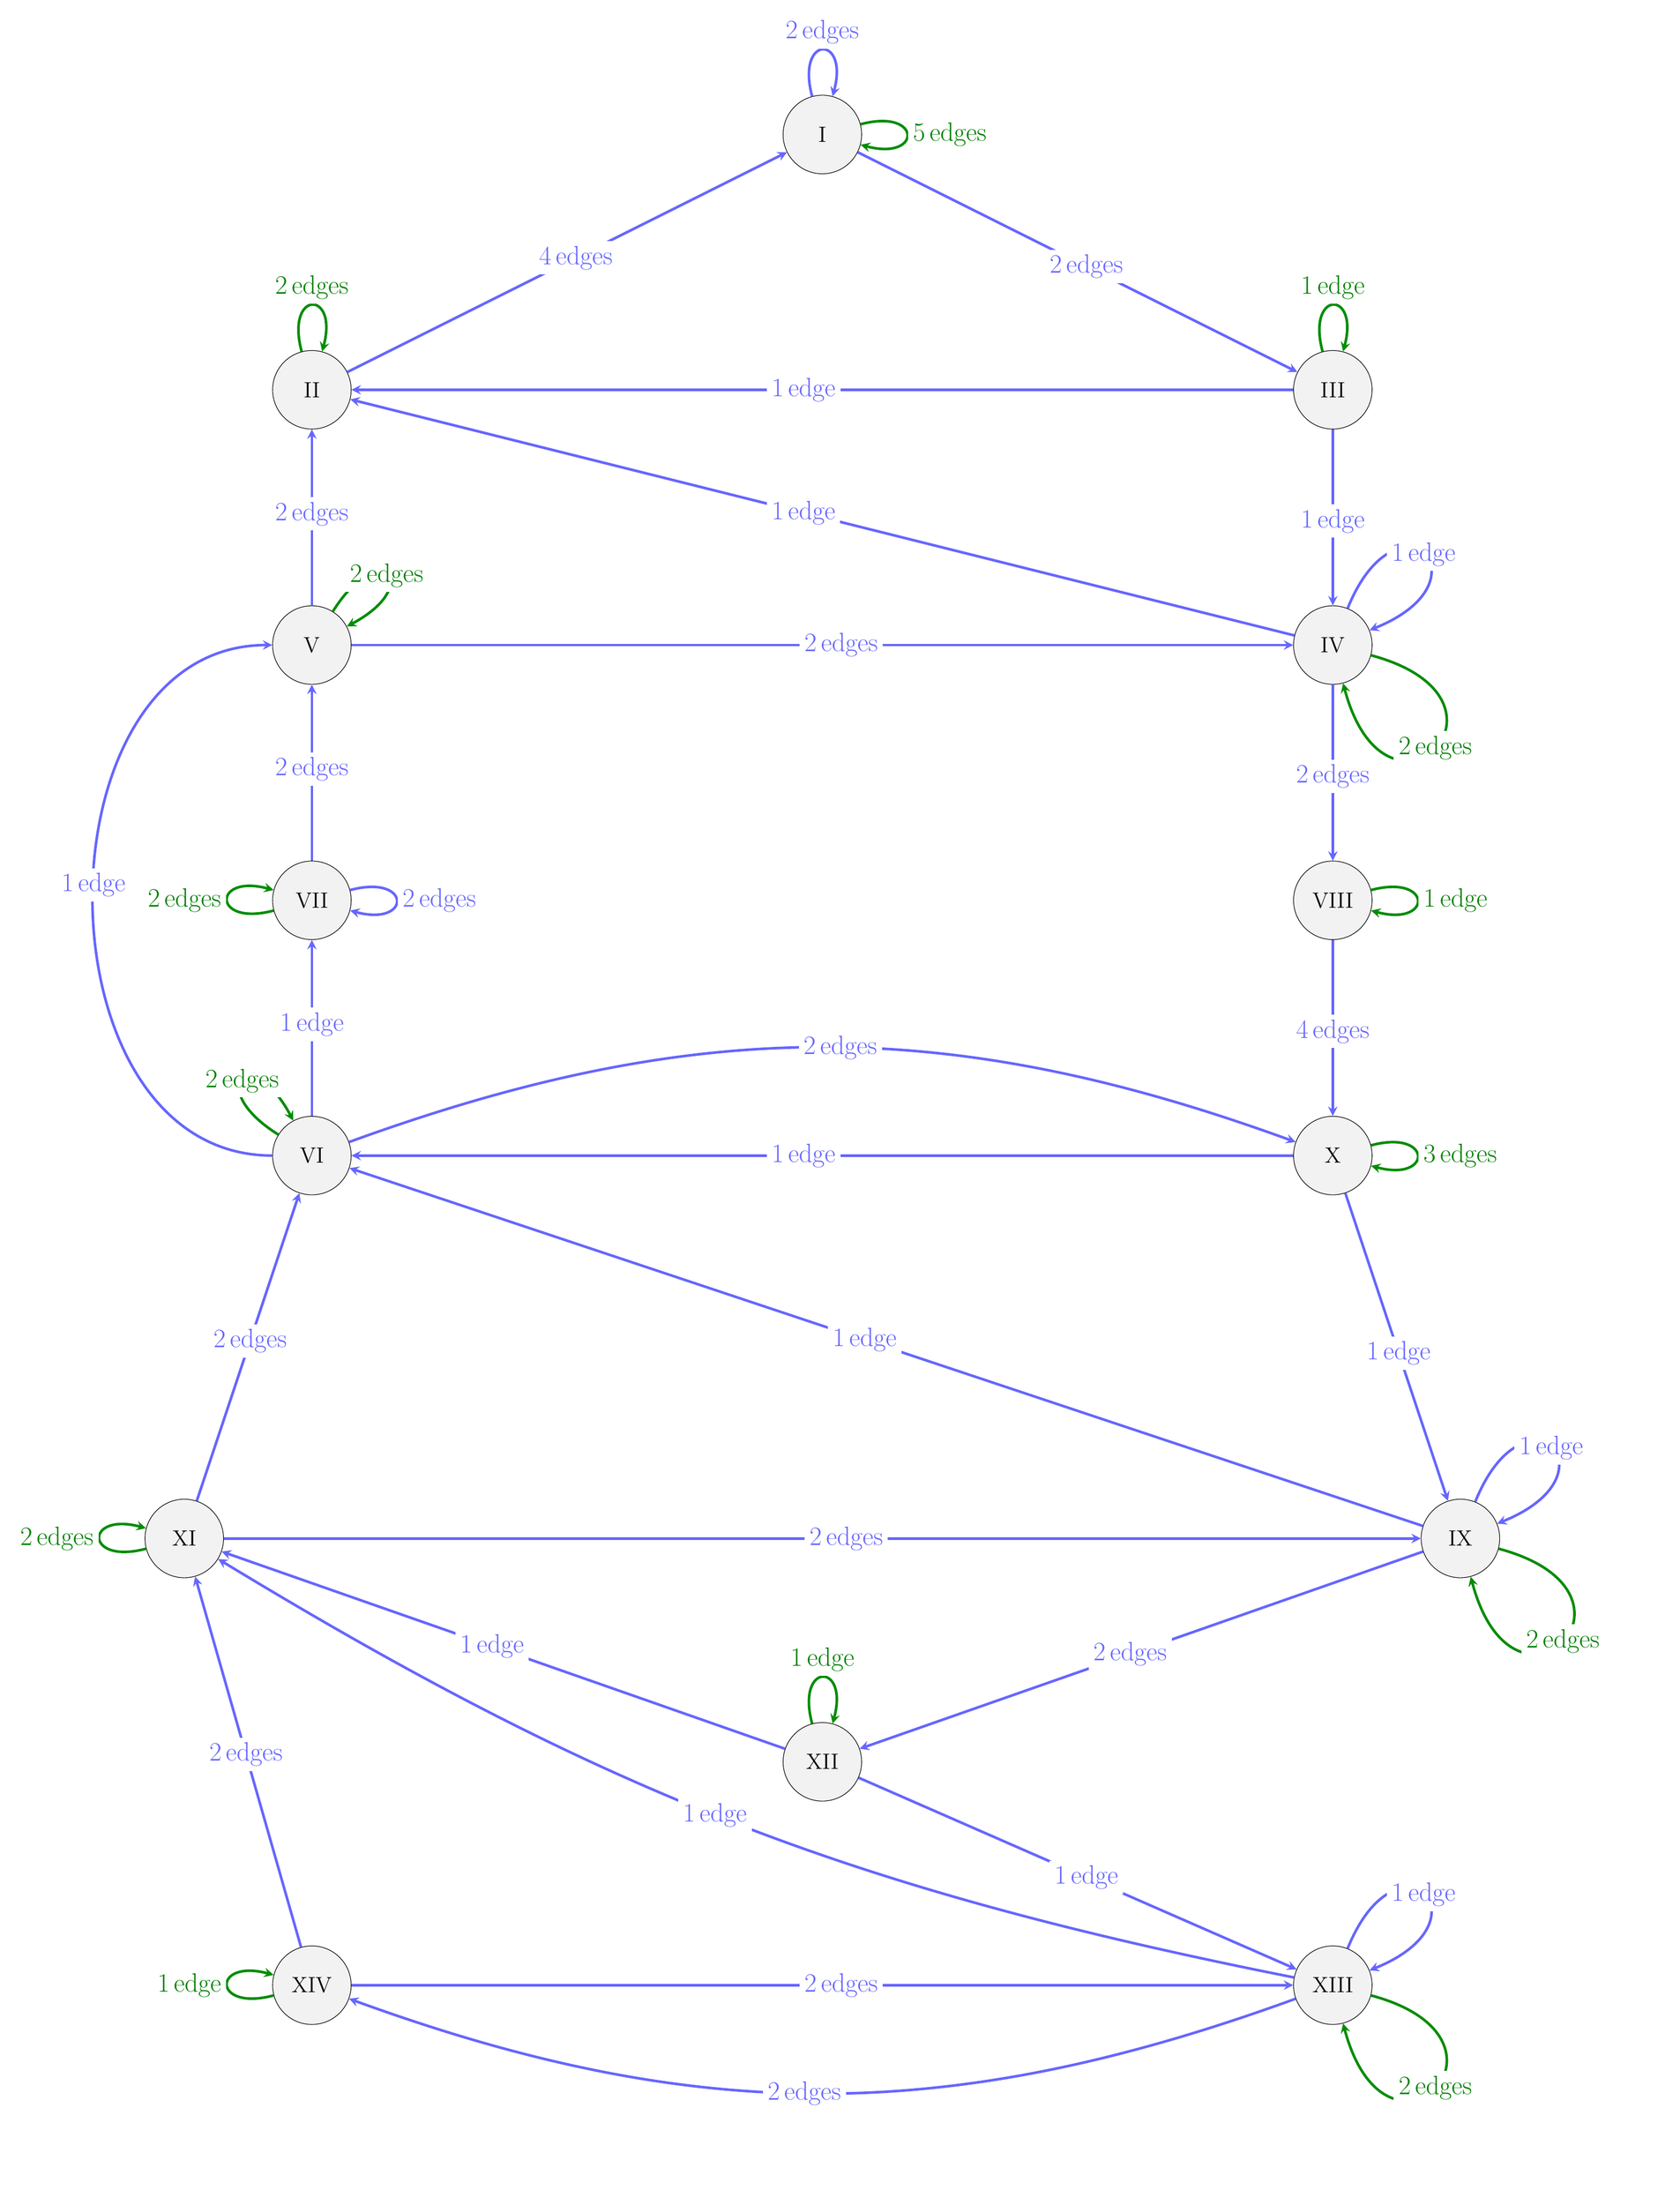
\begin{tikzpicture}[
  >=stealth,
  autnode/.style={circle, draw=black, fill=gray!10, minimum size=18.0mm, inner sep=2.8pt, font={\Large}},
  autedge/.style={->, draw=blue!60, line width=1.70pt},
  autlbl/.style={font={\LARGE}, transform shape, text=blue!60, fill=white, inner sep=3.2pt},
  autedgeperm/.style={->, draw=green!55!black, line width=1.70pt},
  autlblperm/.style={font={\LARGE}, transform shape, text=green!50!black, fill=white, inner sep=3.2pt}
]
\node[autnode] (n1) at (-11.7000,29.2500) {$\mathrm{II}$};
\node[autnode] (n2) at (0.0000,35.1000) {$\mathrm{I}$};
\node[autnode] (n3) at (-11.7000,17.5500) {$\mathrm{VII}$};
\node[autnode] (n4) at (11.7000,17.5500) {$\mathrm{VIII}$};
\node[autnode] (n5) at (-11.7000,11.7000) {$\mathrm{VI}$};
\node[autnode] (n6) at (11.7000,29.2500) {$\mathrm{III}$};
\node[autnode] (n7) at (11.7000,11.7000) {$\mathrm{X}$};
\node[autnode] (n8) at (0.0000,-2.1938) {$\mathrm{XII}$};
\node[autnode] (n9) at (11.7000,23.4000) {$\mathrm{IV}$};
\node[autnode] (n10) at (14.6250,2.9250) {$\mathrm{IX}$};
\node[autnode] (n11) at (11.7000,-7.3125) {$\mathrm{XIII}$};
\node[autnode] (n12) at (-11.7000,23.4000) {$\mathrm{V}$};
\node[autnode] (n13) at (-14.6250,2.9250) {$\mathrm{XI}$};
\node[autnode] (n14) at (-11.7000,-7.3125) {$\mathrm{XIV}$};
\draw[autedgeperm] (n1) to[loop above] node[autlblperm] {$ 2\,\mathrm{edges} $} (n1);
\draw[autedge] (n1) -- node[autlbl, pos=0.52] {$ 4\,\mathrm{edges} $} (n2);
\draw[autedge] (n2) to[loop above] node[autlbl] {$ 2\,\mathrm{edges} $} (n2);
\draw[autedgeperm] (n2) to[loop right] node[autlblperm] {$ 5\,\mathrm{edges} $} (n2);
\draw[autedge] (n2) -- node[autlbl, pos=0.52] {$ 2\,\mathrm{edges} $} (n6);
\draw[autedge] (n3) to[loop right] node[autlbl] {$ 2\,\mathrm{edges} $} (n3);
\draw[autedgeperm] (n3) to[loop left] node[autlblperm] {$ 2\,\mathrm{edges} $} (n3);
\draw[autedge] (n3) -- node[autlbl, pos=0.52] {$ 2\,\mathrm{edges} $} (n12);
\draw[autedgeperm] (n4) to[loop right] node[autlblperm] {$ 1\,\mathrm{edge} $} (n4);
\draw[autedge] (n4) -- node[autlbl, pos=0.52] {$ 4\,\mathrm{edges} $} (n7);
\draw[autedge] (n5) -- node[autlbl, pos=0.52] {$ 1\,\mathrm{edge} $} (n3);
\draw[autedgeperm] (n5) to[out=148,in=118,min distance=18mm,looseness=11] node[autlblperm] {$ 2\,\mathrm{edges} $} (n5);
\draw[autedge] (n5) to[bend left=20] node[autlbl, pos=0.52] {$ 2\,\mathrm{edges} $} (n7);
\draw[autedge] (n7) -- node[autlbl, pos=0.52] {$ 1\,\mathrm{edge} $} (n5);
\draw[autedge] (n5) to[out=180,in=180,looseness=1.2] node[autlbl, pos=0.52] {$ 1\,\mathrm{edge} $} (n12);
\draw[autedge] (n6) -- node[autlbl, pos=0.52] {$ 1\,\mathrm{edge} $} (n1);
\draw[autedgeperm] (n6) to[loop above] node[autlblperm] {$ 1\,\mathrm{edge} $} (n6);
\draw[autedge] (n6) -- node[autlbl, pos=0.52] {$ 1\,\mathrm{edge} $} (n9);
\draw[autedgeperm] (n7) to[loop right] node[autlblperm] {$ 3\,\mathrm{edges} $} (n7);
\draw[autedge] (n7) -- node[autlbl, pos=0.52] {$ 1\,\mathrm{edge} $} (n10);
\draw[autedgeperm] (n8) to[loop above] node[autlblperm] {$ 1\,\mathrm{edge} $} (n8);
\draw[autedge] (n8) -- node[autlbl, pos=0.52] {$ 1\,\mathrm{edge} $} (n11);
\draw[autedge] (n8) -- node[autlbl, pos=0.52] {$ 1\,\mathrm{edge} $} (n13);
\draw[autedge] (n9) -- node[autlbl, pos=0.52] {$ 1\,\mathrm{edge} $} (n1);
\draw[autedge] (n9) -- node[autlbl, pos=0.52] {$ 2\,\mathrm{edges} $} (n4);
\draw[autedge] (n9) to[out=68,in=22,min distance=18mm,looseness=11] node[autlbl] {$ 1\,\mathrm{edge} $} (n9);
\draw[autedgeperm] (n9) to[out=345,in=285,min distance=21.5mm,looseness=11] node[autlblperm] {$ 2\,\mathrm{edges} $} (n9);
\draw[autedge] (n10) -- node[autlbl, pos=0.52] {$ 1\,\mathrm{edge} $} (n5);
\draw[autedge] (n10) -- node[autlbl, pos=0.52] {$ 2\,\mathrm{edges} $} (n8);
\draw[autedge] (n10) to[out=68,in=22,min distance=18mm,looseness=11] node[autlbl] {$ 1\,\mathrm{edge} $} (n10);
\draw[autedgeperm] (n10) to[out=345,in=285,min distance=21.5mm,looseness=11] node[autlblperm] {$ 2\,\mathrm{edges} $} (n10);
\draw[autedge] (n11) to[out=68,in=22,min distance=18mm,looseness=11] node[autlbl] {$ 1\,\mathrm{edge} $} (n11);
\draw[autedgeperm] (n11) to[out=345,in=285,min distance=21.5mm,looseness=11] node[autlblperm] {$ 2\,\mathrm{edges} $} (n11);
\draw[autedge] (n11) to[bend left=10] node[autlbl, pos=0.52] {$ 1\,\mathrm{edge} $} (n13);
\draw[autedge] (n11) to[bend left=20] node[autlbl, pos=0.52] {$ 2\,\mathrm{edges} $} (n14);
\draw[autedge] (n14) -- node[autlbl, pos=0.52] {$ 2\,\mathrm{edges} $} (n11);
\draw[autedge] (n12) -- node[autlbl, pos=0.52] {$ 2\,\mathrm{edges} $} (n1);
\draw[autedge] (n12) -- node[autlbl, pos=0.52] {$ 2\,\mathrm{edges} $} (n9);
\draw[autedgeperm] (n12) to[out=58,in=28,min distance=18mm,looseness=11] node[autlblperm] {$ 2\,\mathrm{edges} $} (n12);
\draw[autedge] (n13) -- node[autlbl, pos=0.52] {$ 2\,\mathrm{edges} $} (n5);
\draw[autedge] (n13) -- node[autlbl, pos=0.52] {$ 2\,\mathrm{edges} $} (n10);
\draw[autedgeperm] (n13) to[loop left] node[autlblperm] {$ 2\,\mathrm{edges} $} (n13);
\draw[autedge] (n14) -- node[autlbl, pos=0.52] {$ 2\,\mathrm{edges} $} (n13);
\draw[autedgeperm] (n14) to[loop left] node[autlblperm] {$ 1\,\mathrm{edge} $} (n14);
\end{tikzpicture}%
}
}%
\ifdim\wd0>\dimexpr 1.0\linewidth\relax
  \resizebox{1.0\linewidth}{!}{\box0}%
\else
  \box0%
\fi
\end{center}

\vfill
\clearpage
\noindent\textit{Node index list for this component.}
\begin{itemize}[leftmargin=*]
\item Box $\mathrm{II}$ $= \mathrm{Class}_{1}\,(\mathrm{II})$.
\item Box $\mathrm{I}$ $= \mathrm{Class}_{2}\,(\mathrm{I})$.
\item Box $\mathrm{VII}$ $= \mathrm{Class}_{3}\,(\mathrm{VII})$.
\item Box $\mathrm{VIII}$ $= \mathrm{Class}_{4}\,(\mathrm{VIII})$.
\item Box $\mathrm{VI}$ $= \mathrm{Class}_{5}\,(\mathrm{VI})$.
\item Box $\mathrm{III}$ $= \mathrm{Class}_{6}\,(\mathrm{III})$.
\item Box $\mathrm{X}$ $= \mathrm{Class}_{7}\,(\mathrm{X})$.
\item Box $\mathrm{XII}$ $= \mathrm{Class}_{8}\,(\mathrm{XII})$.
\item Box $\mathrm{IV}$ $= \mathrm{Class}_{9}\,(\mathrm{IV})$.
\item Box $\mathrm{IX}$ $= \mathrm{Class}_{10}\,(\mathrm{IX})$.
\item Box $\mathrm{XIII}$ $= \mathrm{Class}_{11}\,(\mathrm{XIII})$.
\item Box $\mathrm{V}$ $= \mathrm{Class}_{12}\,(\mathrm{V})$.
\item Box $\mathrm{XI}$ $= \mathrm{Class}_{13}\,(\mathrm{XI})$.
\item Box $\mathrm{XIV}$ $= \mathrm{Class}_{14}\,(\mathrm{XIV})$.
\end{itemize}

\clearpage

\subsection*{Visual depiction of full preAUT (one node per box)}
This is the box-collapsed preAUT: each node is one Roman box (I--XIV). A directed edge is drawn from one box to another whenever preAUT has at least one edge between their corresponding classes. As in the AUT diagrams, blue counts Step~2 transitions only and green counts permutation ($\varphi$) edges along each directed box pair.

\paragraph{Box-collapsed preAUT component 1.}
\begin{center}
\resizebox{1.0000\linewidth}{!}{%
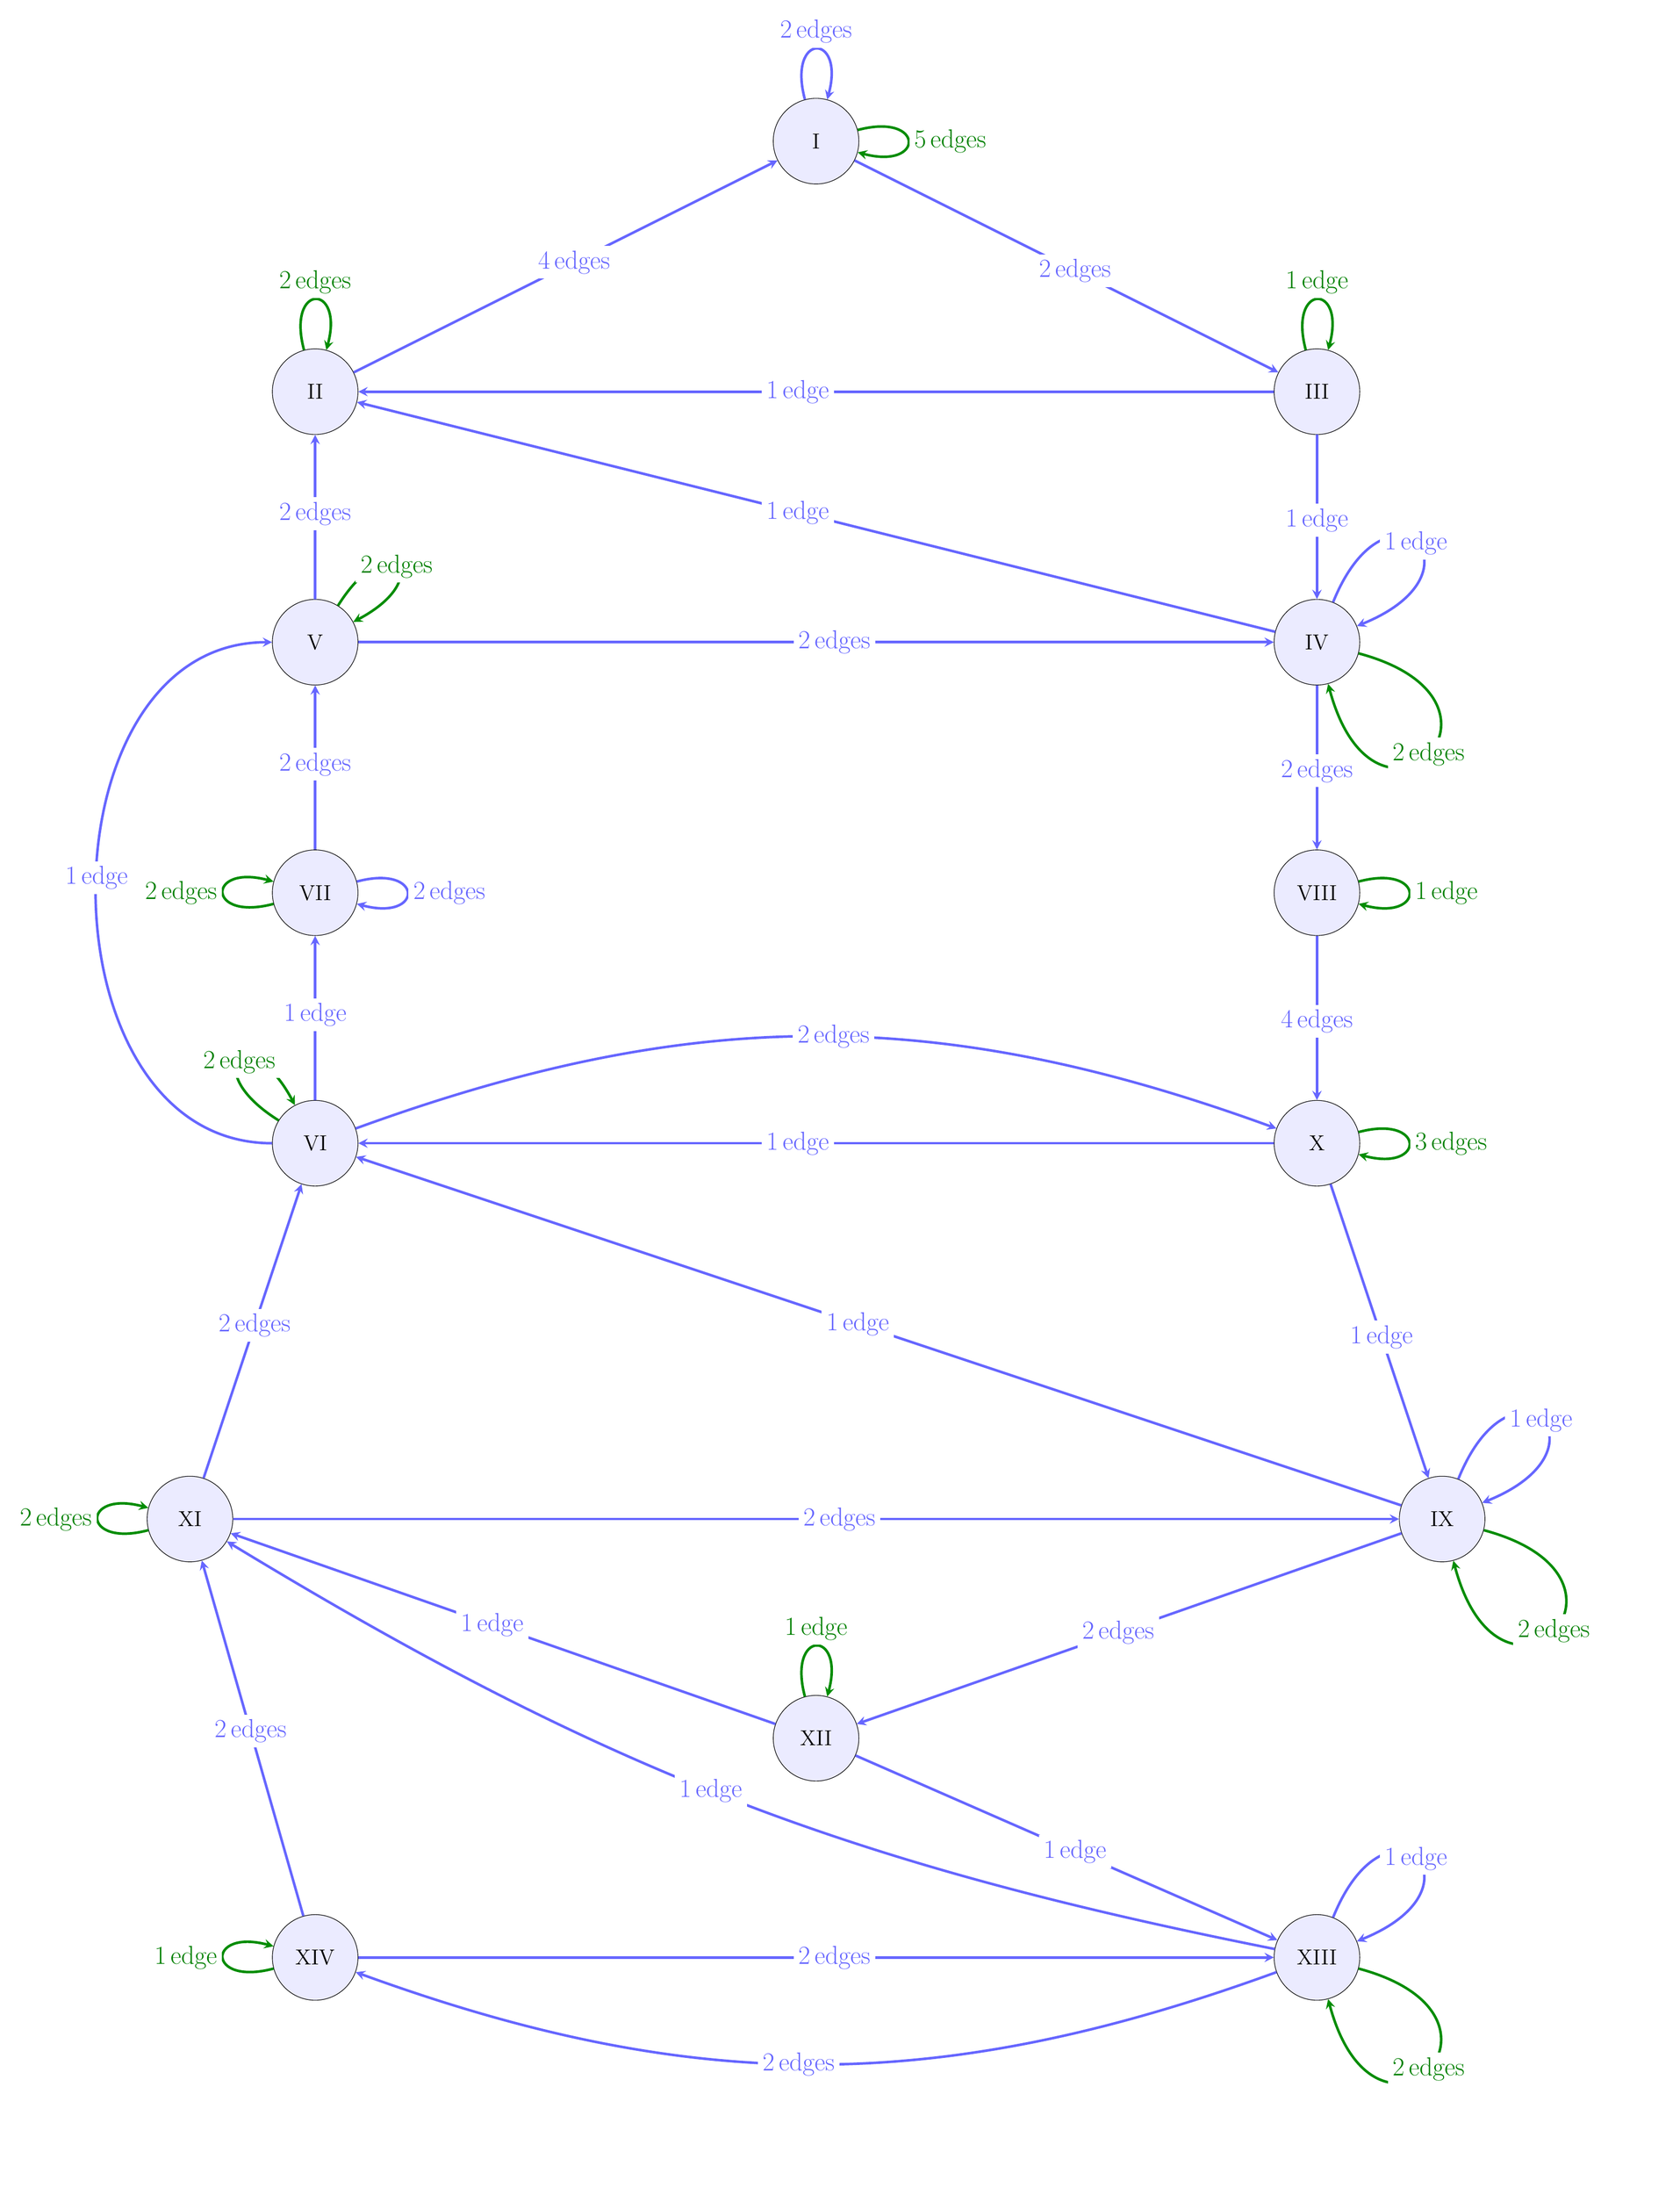
\begin{tikzpicture}[
  >=stealth,
  autnode/.style={circle, draw=black, fill=blue!8, minimum size=20.0mm, inner sep=3.2pt, font={\Large}},
  autedge/.style={->, draw=blue!60, line width=1.70pt},
  autlbl/.style={font={\LARGE}, transform shape, text=blue!60, fill=white, inner sep=3.2pt},
  autedgeperm/.style={->, draw=green!55!black, line width=1.70pt},
  autlblperm/.style={font={\LARGE}, transform shape, text=green!50!black, fill=white, inner sep=3.2pt}
]
\node[autnode] (n1) at (-11.7000,29.2500) {$\mathrm{II}$};
\node[autnode] (n2) at (0.0000,35.1000) {$\mathrm{I}$};
\node[autnode] (n3) at (-11.7000,17.5500) {$\mathrm{VII}$};
\node[autnode] (n4) at (11.7000,17.5500) {$\mathrm{VIII}$};
\node[autnode] (n5) at (-11.7000,11.7000) {$\mathrm{VI}$};
\node[autnode] (n6) at (11.7000,29.2500) {$\mathrm{III}$};
\node[autnode] (n7) at (11.7000,11.7000) {$\mathrm{X}$};
\node[autnode] (n8) at (0.0000,-2.1938) {$\mathrm{XII}$};
\node[autnode] (n9) at (11.7000,23.4000) {$\mathrm{IV}$};
\node[autnode] (n10) at (14.6250,2.9250) {$\mathrm{IX}$};
\node[autnode] (n11) at (11.7000,-7.3125) {$\mathrm{XIII}$};
\node[autnode] (n12) at (-11.7000,23.4000) {$\mathrm{V}$};
\node[autnode] (n13) at (-14.6250,2.9250) {$\mathrm{XI}$};
\node[autnode] (n14) at (-11.7000,-7.3125) {$\mathrm{XIV}$};
\draw[autedgeperm] (n1) to[loop above] node[autlblperm] {$ 2\,\mathrm{edges} $} (n1);
\draw[autedge] (n1) -- node[autlbl, pos=0.52] {$ 4\,\mathrm{edges} $} (n2);
\draw[autedge] (n2) to[loop above] node[autlbl] {$ 2\,\mathrm{edges} $} (n2);
\draw[autedgeperm] (n2) to[loop right] node[autlblperm] {$ 5\,\mathrm{edges} $} (n2);
\draw[autedge] (n2) -- node[autlbl, pos=0.52] {$ 2\,\mathrm{edges} $} (n6);
\draw[autedge] (n3) to[loop right] node[autlbl] {$ 2\,\mathrm{edges} $} (n3);
\draw[autedgeperm] (n3) to[loop left] node[autlblperm] {$ 2\,\mathrm{edges} $} (n3);
\draw[autedge] (n3) -- node[autlbl, pos=0.52] {$ 2\,\mathrm{edges} $} (n12);
\draw[autedgeperm] (n4) to[loop right] node[autlblperm] {$ 1\,\mathrm{edge} $} (n4);
\draw[autedge] (n4) -- node[autlbl, pos=0.52] {$ 4\,\mathrm{edges} $} (n7);
\draw[autedge] (n5) -- node[autlbl, pos=0.52] {$ 1\,\mathrm{edge} $} (n3);
\draw[autedgeperm] (n5) to[out=148,in=118,min distance=18mm,looseness=11] node[autlblperm] {$ 2\,\mathrm{edges} $} (n5);
\draw[autedge] (n5) to[bend left=20] node[autlbl, pos=0.52] {$ 2\,\mathrm{edges} $} (n7);
\draw[autedge] (n7) -- node[autlbl, pos=0.52] {$ 1\,\mathrm{edge} $} (n5);
\draw[autedge] (n5) to[out=180,in=180,looseness=1.2] node[autlbl, pos=0.52] {$ 1\,\mathrm{edge} $} (n12);
\draw[autedge] (n6) -- node[autlbl, pos=0.52] {$ 1\,\mathrm{edge} $} (n1);
\draw[autedgeperm] (n6) to[loop above] node[autlblperm] {$ 1\,\mathrm{edge} $} (n6);
\draw[autedge] (n6) -- node[autlbl, pos=0.52] {$ 1\,\mathrm{edge} $} (n9);
\draw[autedgeperm] (n7) to[loop right] node[autlblperm] {$ 3\,\mathrm{edges} $} (n7);
\draw[autedge] (n7) -- node[autlbl, pos=0.52] {$ 1\,\mathrm{edge} $} (n10);
\draw[autedgeperm] (n8) to[loop above] node[autlblperm] {$ 1\,\mathrm{edge} $} (n8);
\draw[autedge] (n8) -- node[autlbl, pos=0.52] {$ 1\,\mathrm{edge} $} (n11);
\draw[autedge] (n8) -- node[autlbl, pos=0.52] {$ 1\,\mathrm{edge} $} (n13);
\draw[autedge] (n9) -- node[autlbl, pos=0.52] {$ 1\,\mathrm{edge} $} (n1);
\draw[autedge] (n9) -- node[autlbl, pos=0.52] {$ 2\,\mathrm{edges} $} (n4);
\draw[autedge] (n9) to[out=68,in=22,min distance=18mm,looseness=11] node[autlbl] {$ 1\,\mathrm{edge} $} (n9);
\draw[autedgeperm] (n9) to[out=345,in=285,min distance=21.5mm,looseness=11] node[autlblperm] {$ 2\,\mathrm{edges} $} (n9);
\draw[autedge] (n10) -- node[autlbl, pos=0.52] {$ 1\,\mathrm{edge} $} (n5);
\draw[autedge] (n10) -- node[autlbl, pos=0.52] {$ 2\,\mathrm{edges} $} (n8);
\draw[autedge] (n10) to[out=68,in=22,min distance=18mm,looseness=11] node[autlbl] {$ 1\,\mathrm{edge} $} (n10);
\draw[autedgeperm] (n10) to[out=345,in=285,min distance=21.5mm,looseness=11] node[autlblperm] {$ 2\,\mathrm{edges} $} (n10);
\draw[autedge] (n11) to[out=68,in=22,min distance=18mm,looseness=11] node[autlbl] {$ 1\,\mathrm{edge} $} (n11);
\draw[autedgeperm] (n11) to[out=345,in=285,min distance=21.5mm,looseness=11] node[autlblperm] {$ 2\,\mathrm{edges} $} (n11);
\draw[autedge] (n11) to[bend left=10] node[autlbl, pos=0.52] {$ 1\,\mathrm{edge} $} (n13);
\draw[autedge] (n11) to[bend left=20] node[autlbl, pos=0.52] {$ 2\,\mathrm{edges} $} (n14);
\draw[autedge] (n14) -- node[autlbl, pos=0.52] {$ 2\,\mathrm{edges} $} (n11);
\draw[autedge] (n12) -- node[autlbl, pos=0.52] {$ 2\,\mathrm{edges} $} (n1);
\draw[autedge] (n12) -- node[autlbl, pos=0.52] {$ 2\,\mathrm{edges} $} (n9);
\draw[autedgeperm] (n12) to[out=58,in=28,min distance=18mm,looseness=11] node[autlblperm] {$ 2\,\mathrm{edges} $} (n12);
\draw[autedge] (n13) -- node[autlbl, pos=0.52] {$ 2\,\mathrm{edges} $} (n5);
\draw[autedge] (n13) -- node[autlbl, pos=0.52] {$ 2\,\mathrm{edges} $} (n10);
\draw[autedgeperm] (n13) to[loop left] node[autlblperm] {$ 2\,\mathrm{edges} $} (n13);
\draw[autedge] (n14) -- node[autlbl, pos=0.52] {$ 2\,\mathrm{edges} $} (n13);
\draw[autedgeperm] (n14) to[loop left] node[autlblperm] {$ 1\,\mathrm{edge} $} (n14);
\end{tikzpicture}%
}
\end{center}

\noindent\textit{Box index list for this preAUT diagram.}
\begin{itemize}[leftmargin=*]
\item Box $\mathrm{II}$ $= \mathrm{graphs}_{1}=\{G_{26}, G_{29}, G_{5}\}$.
\item Box $\mathrm{I}$ $= \mathrm{graphs}_{2}=\{G, G_{2}, G_{4}, G_{7}, G_{8}, G_{9}\}$.
\item Box $\mathrm{VII}$ $= \mathrm{graphs}_{3}=\{G_{18}, G_{22}, G_{23}\}$.
\item Box $\mathrm{VIII}$ $= \mathrm{graphs}_{4}=\{G_{10}, G_{11}\}$.
\item Box $\mathrm{VI}$ $= \mathrm{graphs}_{5}=\{G_{16}, G_{34}, G_{35}\}$.
\item Box $\mathrm{III}$ $= \mathrm{graphs}_{6}=\{G_{1}, G_{3}\}$.
\item Box $\mathrm{X}$ $= \mathrm{graphs}_{7}=\{G_{12}, G_{13}, G_{14}, G_{15}\}$.
\item Box $\mathrm{XII}$ $= \mathrm{graphs}_{8}=\{G_{20}, G_{21}\}$.
\item Box $\mathrm{IV}$ $= \mathrm{graphs}_{9}=\{G_{27}, G_{28}, G_{6}\}$.
\item Box $\mathrm{IX}$ $= \mathrm{graphs}_{10}=\{G_{17}, G_{36}, G_{37}\}$.
\item Box $\mathrm{XIII}$ $= \mathrm{graphs}_{11}=\{G_{30}, G_{38}, G_{39}\}$.
\item Box $\mathrm{V}$ $= \mathrm{graphs}_{12}=\{G_{19}, G_{24}, G_{25}\}$.
\item Box $\mathrm{XI}$ $= \mathrm{graphs}_{13}=\{G_{31}, G_{40}, G_{41}\}$.
\item Box $\mathrm{XIV}$ $= \mathrm{graphs}_{14}=\{G_{32}, G_{33}\}$.
\end{itemize}


\subsection*{preAUT edges omitted in AUT (cross-SCC/exiting edges)}
The AUT figures keep only edges whose source and target are in the same maximal SCC. The following preAUT edges leave those SCCs and are therefore omitted from AUT.

\begin{enumerate}[leftmargin=*]
\item From $\mathrm{SCC}_{1}$:
none.
\end{enumerate}

\subsection*{Visual depiction of omitted preAUT edges by SCC}
For each AUT component $\mathrm{SCC}_i$, we draw the edges that start in $\mathrm{SCC}_i$ and leave it in preAUT. Internal AUT edges are omitted in these diagrams.

\paragraph{Omitted preAUT edges from $\mathrm{SCC}_{1}$.}
\noindent None.


\subsection*{Step 6: coverage check across ep-isomorphism classes}
Covered ep-isomorphism classes: $14$ out of $14$. All classes are represented by the constructed preAUT, so no additional seed run is required.

\subsection*{Step 7: maximal SCCs and AUT (box-collapsed)}
Each maximal strongly connected component (SCC) of the box-collapsed preAUT is listed below; AUT is their disjoint union.

\paragraph{SCC decomposition of preAUT.}
\begin{enumerate}[leftmargin=*]
\item $\mathrm{SCC}_{1}=\{\mathrm{Class}_{1}\,(\mathrm{II}), \mathrm{Class}_{10}\,(\mathrm{IX}), \mathrm{Class}_{11}\,(\mathrm{XIII}), \mathrm{Class}_{12}\,(\mathrm{V}), \mathrm{Class}_{13}\,(\mathrm{XI}), \mathrm{Class}_{14}\,(\mathrm{XIV}), \mathrm{Class}_{2}\,(\mathrm{I}), \mathrm{Class}_{3}\,(\mathrm{VII}), \mathrm{Class}_{4}\,(\mathrm{VIII}), \mathrm{Class}_{5}\,(\mathrm{VI}), \mathrm{Class}_{6}\,(\mathrm{III}), \mathrm{Class}_{7}\,(\mathrm{X}), \mathrm{Class}_{8}\,(\mathrm{XII}), \mathrm{Class}_{9}\,(\mathrm{IV})\}$.
\end{enumerate}

\paragraph{Directed edges of AUT.}
These are exactly the box-collapsed preAUT edges whose endpoints lie in the same maximal SCC.
\begin{enumerate}[leftmargin=*]
\item $\mathrm{Class}_{1}\,(\mathrm{II}) \xrightarrow{2\,\mathrm{edges}} \mathrm{Class}_{1}\,(\mathrm{II})$ (inside $\mathrm{SCC}_{1}$).
\item $\mathrm{Class}_{1}\,(\mathrm{II}) \xrightarrow{4\,\mathrm{edges}} \mathrm{Class}_{2}\,(\mathrm{I})$ (inside $\mathrm{SCC}_{1}$).
\item $\mathrm{Class}_{2}\,(\mathrm{I}) \xrightarrow{7\,\mathrm{edges}} \mathrm{Class}_{2}\,(\mathrm{I})$ (inside $\mathrm{SCC}_{1}$).
\item $\mathrm{Class}_{2}\,(\mathrm{I}) \xrightarrow{2\,\mathrm{edges}} \mathrm{Class}_{6}\,(\mathrm{III})$ (inside $\mathrm{SCC}_{1}$).
\item $\mathrm{Class}_{3}\,(\mathrm{VII}) \xrightarrow{4\,\mathrm{edges}} \mathrm{Class}_{3}\,(\mathrm{VII})$ (inside $\mathrm{SCC}_{1}$).
\item $\mathrm{Class}_{3}\,(\mathrm{VII}) \xrightarrow{2\,\mathrm{edges}} \mathrm{Class}_{12}\,(\mathrm{V})$ (inside $\mathrm{SCC}_{1}$).
\item $\mathrm{Class}_{4}\,(\mathrm{VIII}) \xrightarrow{1\,\mathrm{edge}} \mathrm{Class}_{4}\,(\mathrm{VIII})$ (inside $\mathrm{SCC}_{1}$).
\item $\mathrm{Class}_{4}\,(\mathrm{VIII}) \xrightarrow{4\,\mathrm{edges}} \mathrm{Class}_{7}\,(\mathrm{X})$ (inside $\mathrm{SCC}_{1}$).
\item $\mathrm{Class}_{5}\,(\mathrm{VI}) \xrightarrow{1\,\mathrm{edge}} \mathrm{Class}_{3}\,(\mathrm{VII})$ (inside $\mathrm{SCC}_{1}$).
\item $\mathrm{Class}_{5}\,(\mathrm{VI}) \xrightarrow{2\,\mathrm{edges}} \mathrm{Class}_{5}\,(\mathrm{VI})$ (inside $\mathrm{SCC}_{1}$).
\item $\mathrm{Class}_{5}\,(\mathrm{VI}) \xrightarrow{2\,\mathrm{edges}} \mathrm{Class}_{7}\,(\mathrm{X})$ (inside $\mathrm{SCC}_{1}$).
\item $\mathrm{Class}_{5}\,(\mathrm{VI}) \xrightarrow{1\,\mathrm{edge}} \mathrm{Class}_{12}\,(\mathrm{V})$ (inside $\mathrm{SCC}_{1}$).
\item $\mathrm{Class}_{6}\,(\mathrm{III}) \xrightarrow{1\,\mathrm{edge}} \mathrm{Class}_{1}\,(\mathrm{II})$ (inside $\mathrm{SCC}_{1}$).
\item $\mathrm{Class}_{6}\,(\mathrm{III}) \xrightarrow{1\,\mathrm{edge}} \mathrm{Class}_{6}\,(\mathrm{III})$ (inside $\mathrm{SCC}_{1}$).
\item $\mathrm{Class}_{6}\,(\mathrm{III}) \xrightarrow{1\,\mathrm{edge}} \mathrm{Class}_{9}\,(\mathrm{IV})$ (inside $\mathrm{SCC}_{1}$).
\item $\mathrm{Class}_{7}\,(\mathrm{X}) \xrightarrow{1\,\mathrm{edge}} \mathrm{Class}_{5}\,(\mathrm{VI})$ (inside $\mathrm{SCC}_{1}$).
\item $\mathrm{Class}_{7}\,(\mathrm{X}) \xrightarrow{3\,\mathrm{edges}} \mathrm{Class}_{7}\,(\mathrm{X})$ (inside $\mathrm{SCC}_{1}$).
\item $\mathrm{Class}_{7}\,(\mathrm{X}) \xrightarrow{1\,\mathrm{edge}} \mathrm{Class}_{10}\,(\mathrm{IX})$ (inside $\mathrm{SCC}_{1}$).
\item $\mathrm{Class}_{8}\,(\mathrm{XII}) \xrightarrow{1\,\mathrm{edge}} \mathrm{Class}_{8}\,(\mathrm{XII})$ (inside $\mathrm{SCC}_{1}$).
\item $\mathrm{Class}_{8}\,(\mathrm{XII}) \xrightarrow{1\,\mathrm{edge}} \mathrm{Class}_{11}\,(\mathrm{XIII})$ (inside $\mathrm{SCC}_{1}$).
\item $\mathrm{Class}_{8}\,(\mathrm{XII}) \xrightarrow{1\,\mathrm{edge}} \mathrm{Class}_{13}\,(\mathrm{XI})$ (inside $\mathrm{SCC}_{1}$).
\item $\mathrm{Class}_{9}\,(\mathrm{IV}) \xrightarrow{1\,\mathrm{edge}} \mathrm{Class}_{1}\,(\mathrm{II})$ (inside $\mathrm{SCC}_{1}$).
\item $\mathrm{Class}_{9}\,(\mathrm{IV}) \xrightarrow{2\,\mathrm{edges}} \mathrm{Class}_{4}\,(\mathrm{VIII})$ (inside $\mathrm{SCC}_{1}$).
\item $\mathrm{Class}_{9}\,(\mathrm{IV}) \xrightarrow{3\,\mathrm{edges}} \mathrm{Class}_{9}\,(\mathrm{IV})$ (inside $\mathrm{SCC}_{1}$).
\item $\mathrm{Class}_{10}\,(\mathrm{IX}) \xrightarrow{1\,\mathrm{edge}} \mathrm{Class}_{5}\,(\mathrm{VI})$ (inside $\mathrm{SCC}_{1}$).
\item $\mathrm{Class}_{10}\,(\mathrm{IX}) \xrightarrow{2\,\mathrm{edges}} \mathrm{Class}_{8}\,(\mathrm{XII})$ (inside $\mathrm{SCC}_{1}$).
\item $\mathrm{Class}_{10}\,(\mathrm{IX}) \xrightarrow{3\,\mathrm{edges}} \mathrm{Class}_{10}\,(\mathrm{IX})$ (inside $\mathrm{SCC}_{1}$).
\item $\mathrm{Class}_{11}\,(\mathrm{XIII}) \xrightarrow{3\,\mathrm{edges}} \mathrm{Class}_{11}\,(\mathrm{XIII})$ (inside $\mathrm{SCC}_{1}$).
\item $\mathrm{Class}_{11}\,(\mathrm{XIII}) \xrightarrow{1\,\mathrm{edge}} \mathrm{Class}_{13}\,(\mathrm{XI})$ (inside $\mathrm{SCC}_{1}$).
\item $\mathrm{Class}_{11}\,(\mathrm{XIII}) \xrightarrow{2\,\mathrm{edges}} \mathrm{Class}_{14}\,(\mathrm{XIV})$ (inside $\mathrm{SCC}_{1}$).
\item $\mathrm{Class}_{12}\,(\mathrm{V}) \xrightarrow{2\,\mathrm{edges}} \mathrm{Class}_{1}\,(\mathrm{II})$ (inside $\mathrm{SCC}_{1}$).
\item $\mathrm{Class}_{12}\,(\mathrm{V}) \xrightarrow{2\,\mathrm{edges}} \mathrm{Class}_{9}\,(\mathrm{IV})$ (inside $\mathrm{SCC}_{1}$).
\item $\mathrm{Class}_{12}\,(\mathrm{V}) \xrightarrow{2\,\mathrm{edges}} \mathrm{Class}_{12}\,(\mathrm{V})$ (inside $\mathrm{SCC}_{1}$).
\item $\mathrm{Class}_{13}\,(\mathrm{XI}) \xrightarrow{2\,\mathrm{edges}} \mathrm{Class}_{5}\,(\mathrm{VI})$ (inside $\mathrm{SCC}_{1}$).
\item $\mathrm{Class}_{13}\,(\mathrm{XI}) \xrightarrow{2\,\mathrm{edges}} \mathrm{Class}_{10}\,(\mathrm{IX})$ (inside $\mathrm{SCC}_{1}$).
\item $\mathrm{Class}_{13}\,(\mathrm{XI}) \xrightarrow{2\,\mathrm{edges}} \mathrm{Class}_{13}\,(\mathrm{XI})$ (inside $\mathrm{SCC}_{1}$).
\item $\mathrm{Class}_{14}\,(\mathrm{XIV}) \xrightarrow{2\,\mathrm{edges}} \mathrm{Class}_{11}\,(\mathrm{XIII})$ (inside $\mathrm{SCC}_{1}$).
\item $\mathrm{Class}_{14}\,(\mathrm{XIV}) \xrightarrow{2\,\mathrm{edges}} \mathrm{Class}_{13}\,(\mathrm{XI})$ (inside $\mathrm{SCC}_{1}$).
\item $\mathrm{Class}_{14}\,(\mathrm{XIV}) \xrightarrow{1\,\mathrm{edge}} \mathrm{Class}_{14}\,(\mathrm{XIV})$ (inside $\mathrm{SCC}_{1}$).
\end{enumerate}
